\begin{figure}[p]
  \centering
  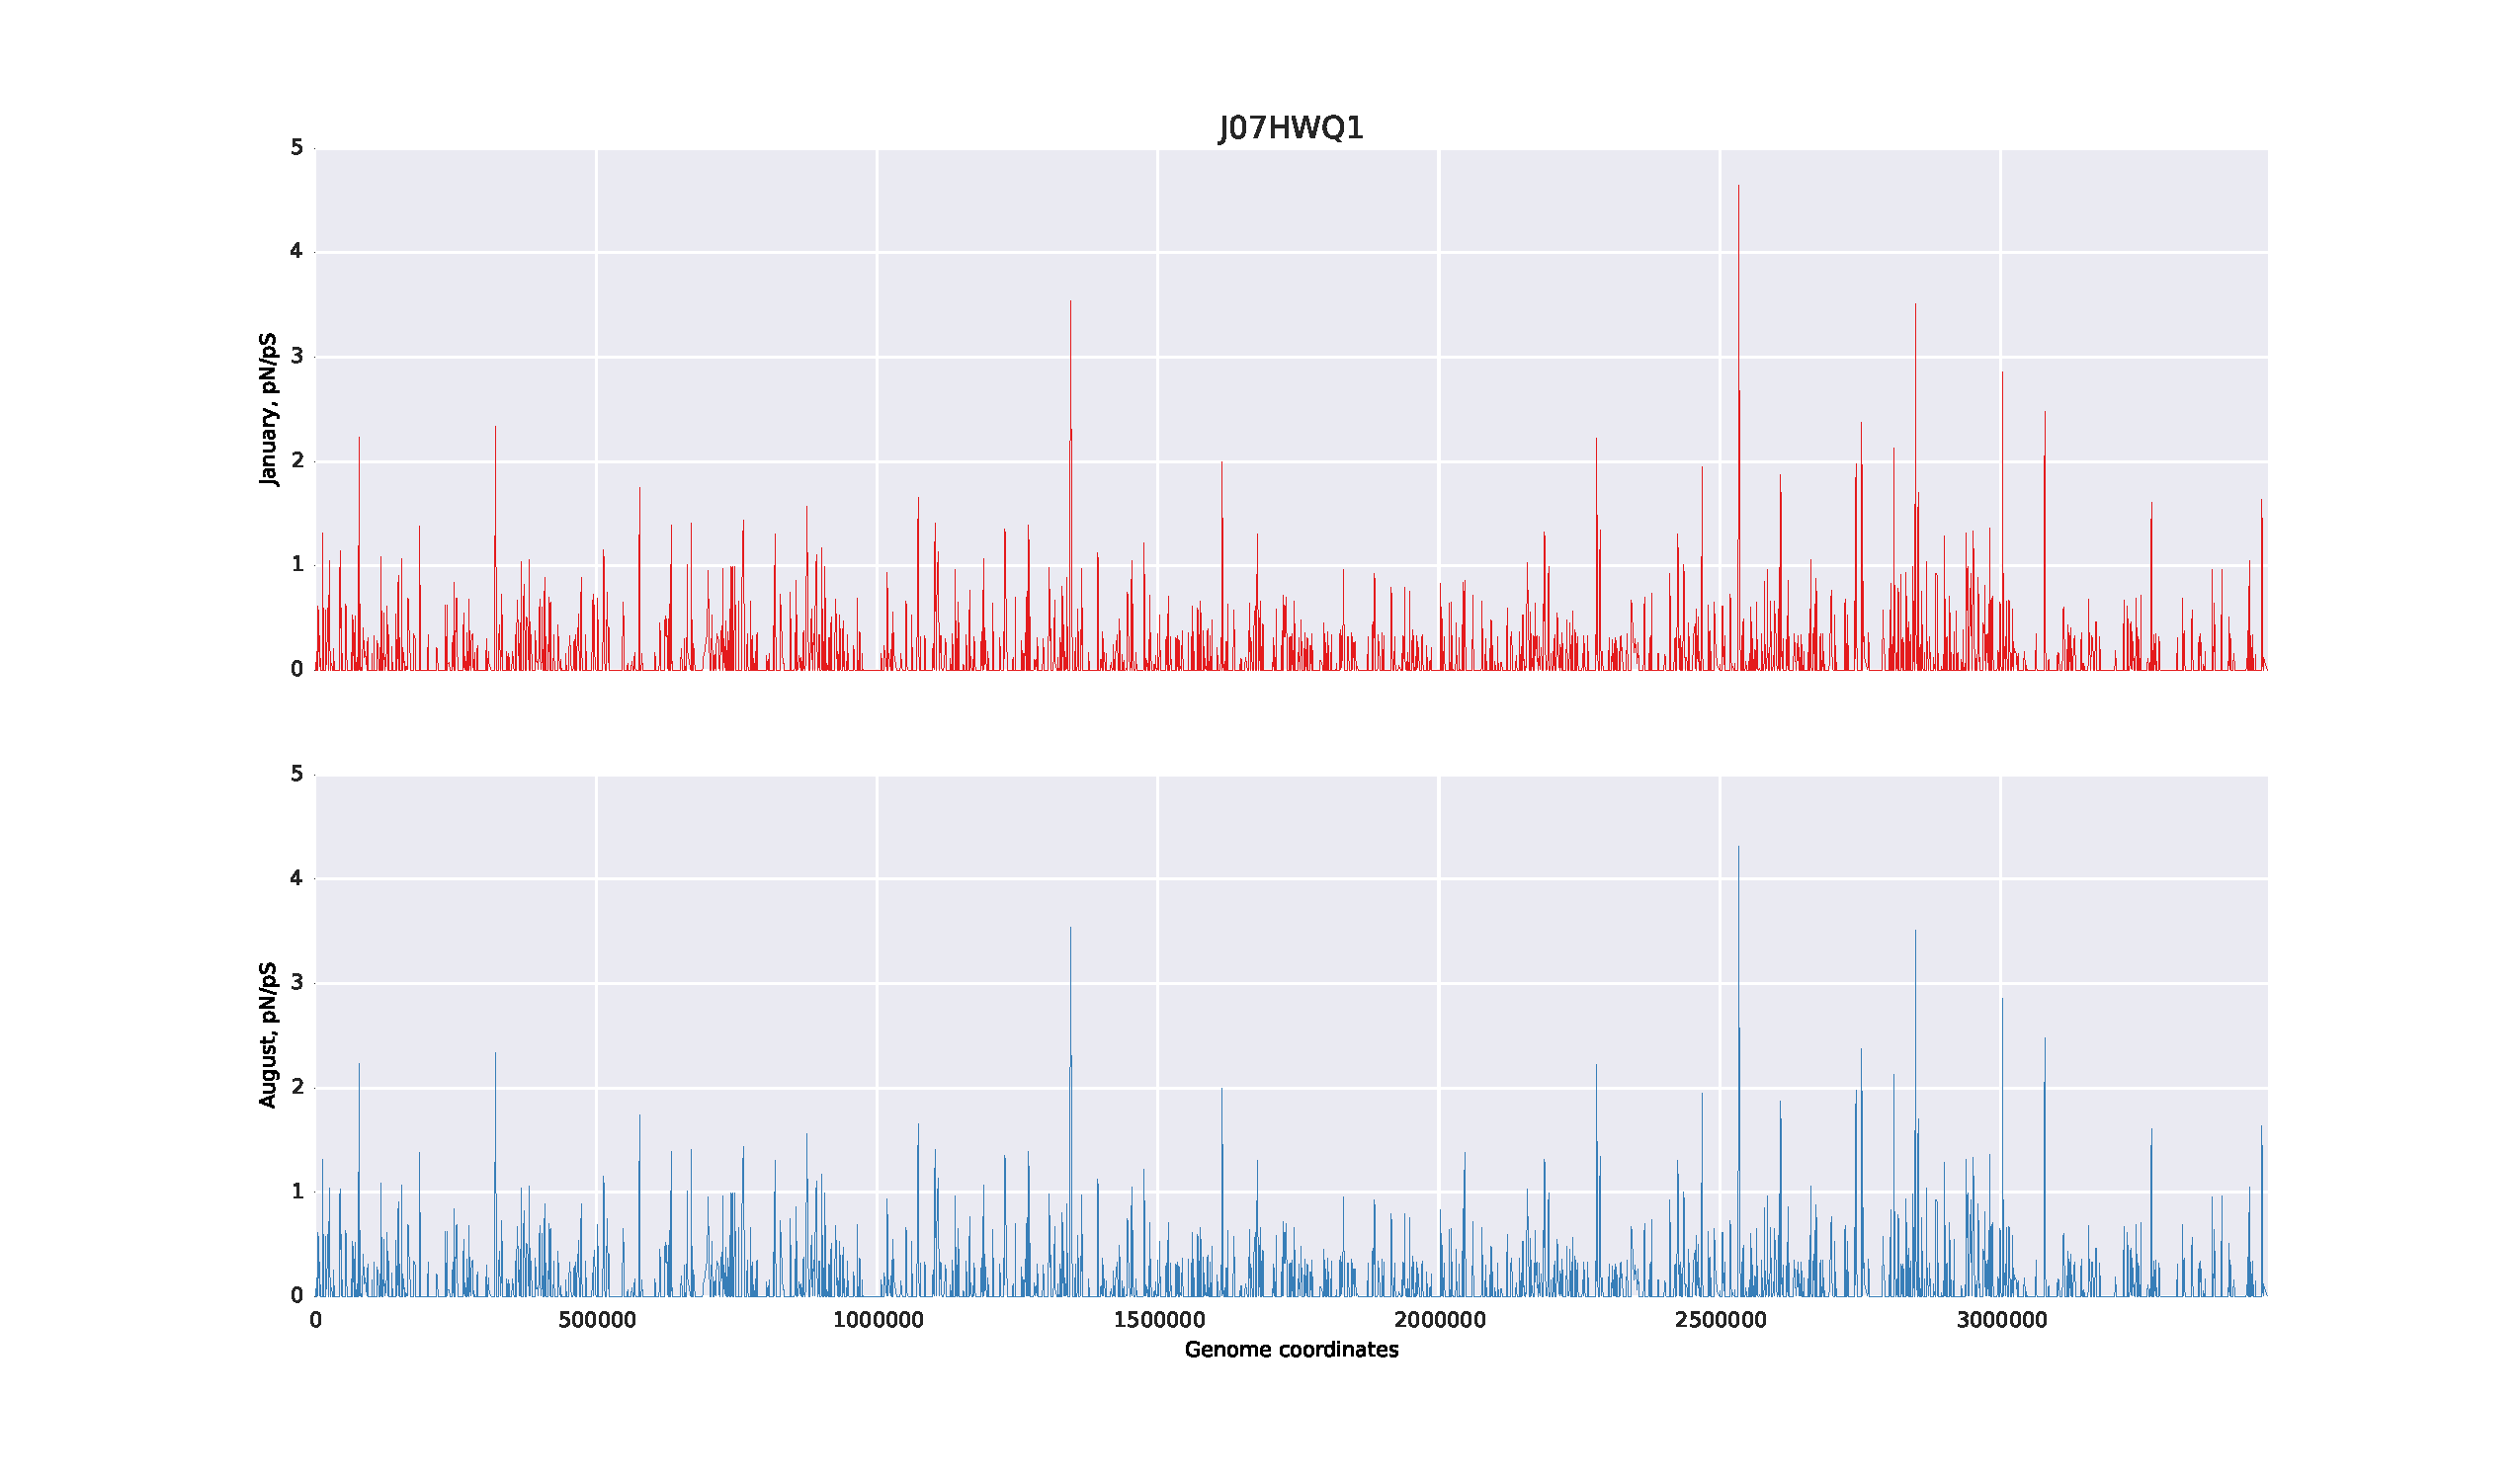
\includegraphics[width=\textwidth,height=\textheight,keepaspectratio]{Chapter5/Figures/pn_ps_plots/J07HWQ1_pNpS_density.pdf}
  \caption{pN/pS values for each gene in the J07HWQ1 genome. Top panel shows the values using the reads from the January samples. Bottom panel shows the values using the reads from the August sample.}
  \label{J07HWQ1_pNpS}
\end{figure}

\begin{figure}[p]
  \centering
  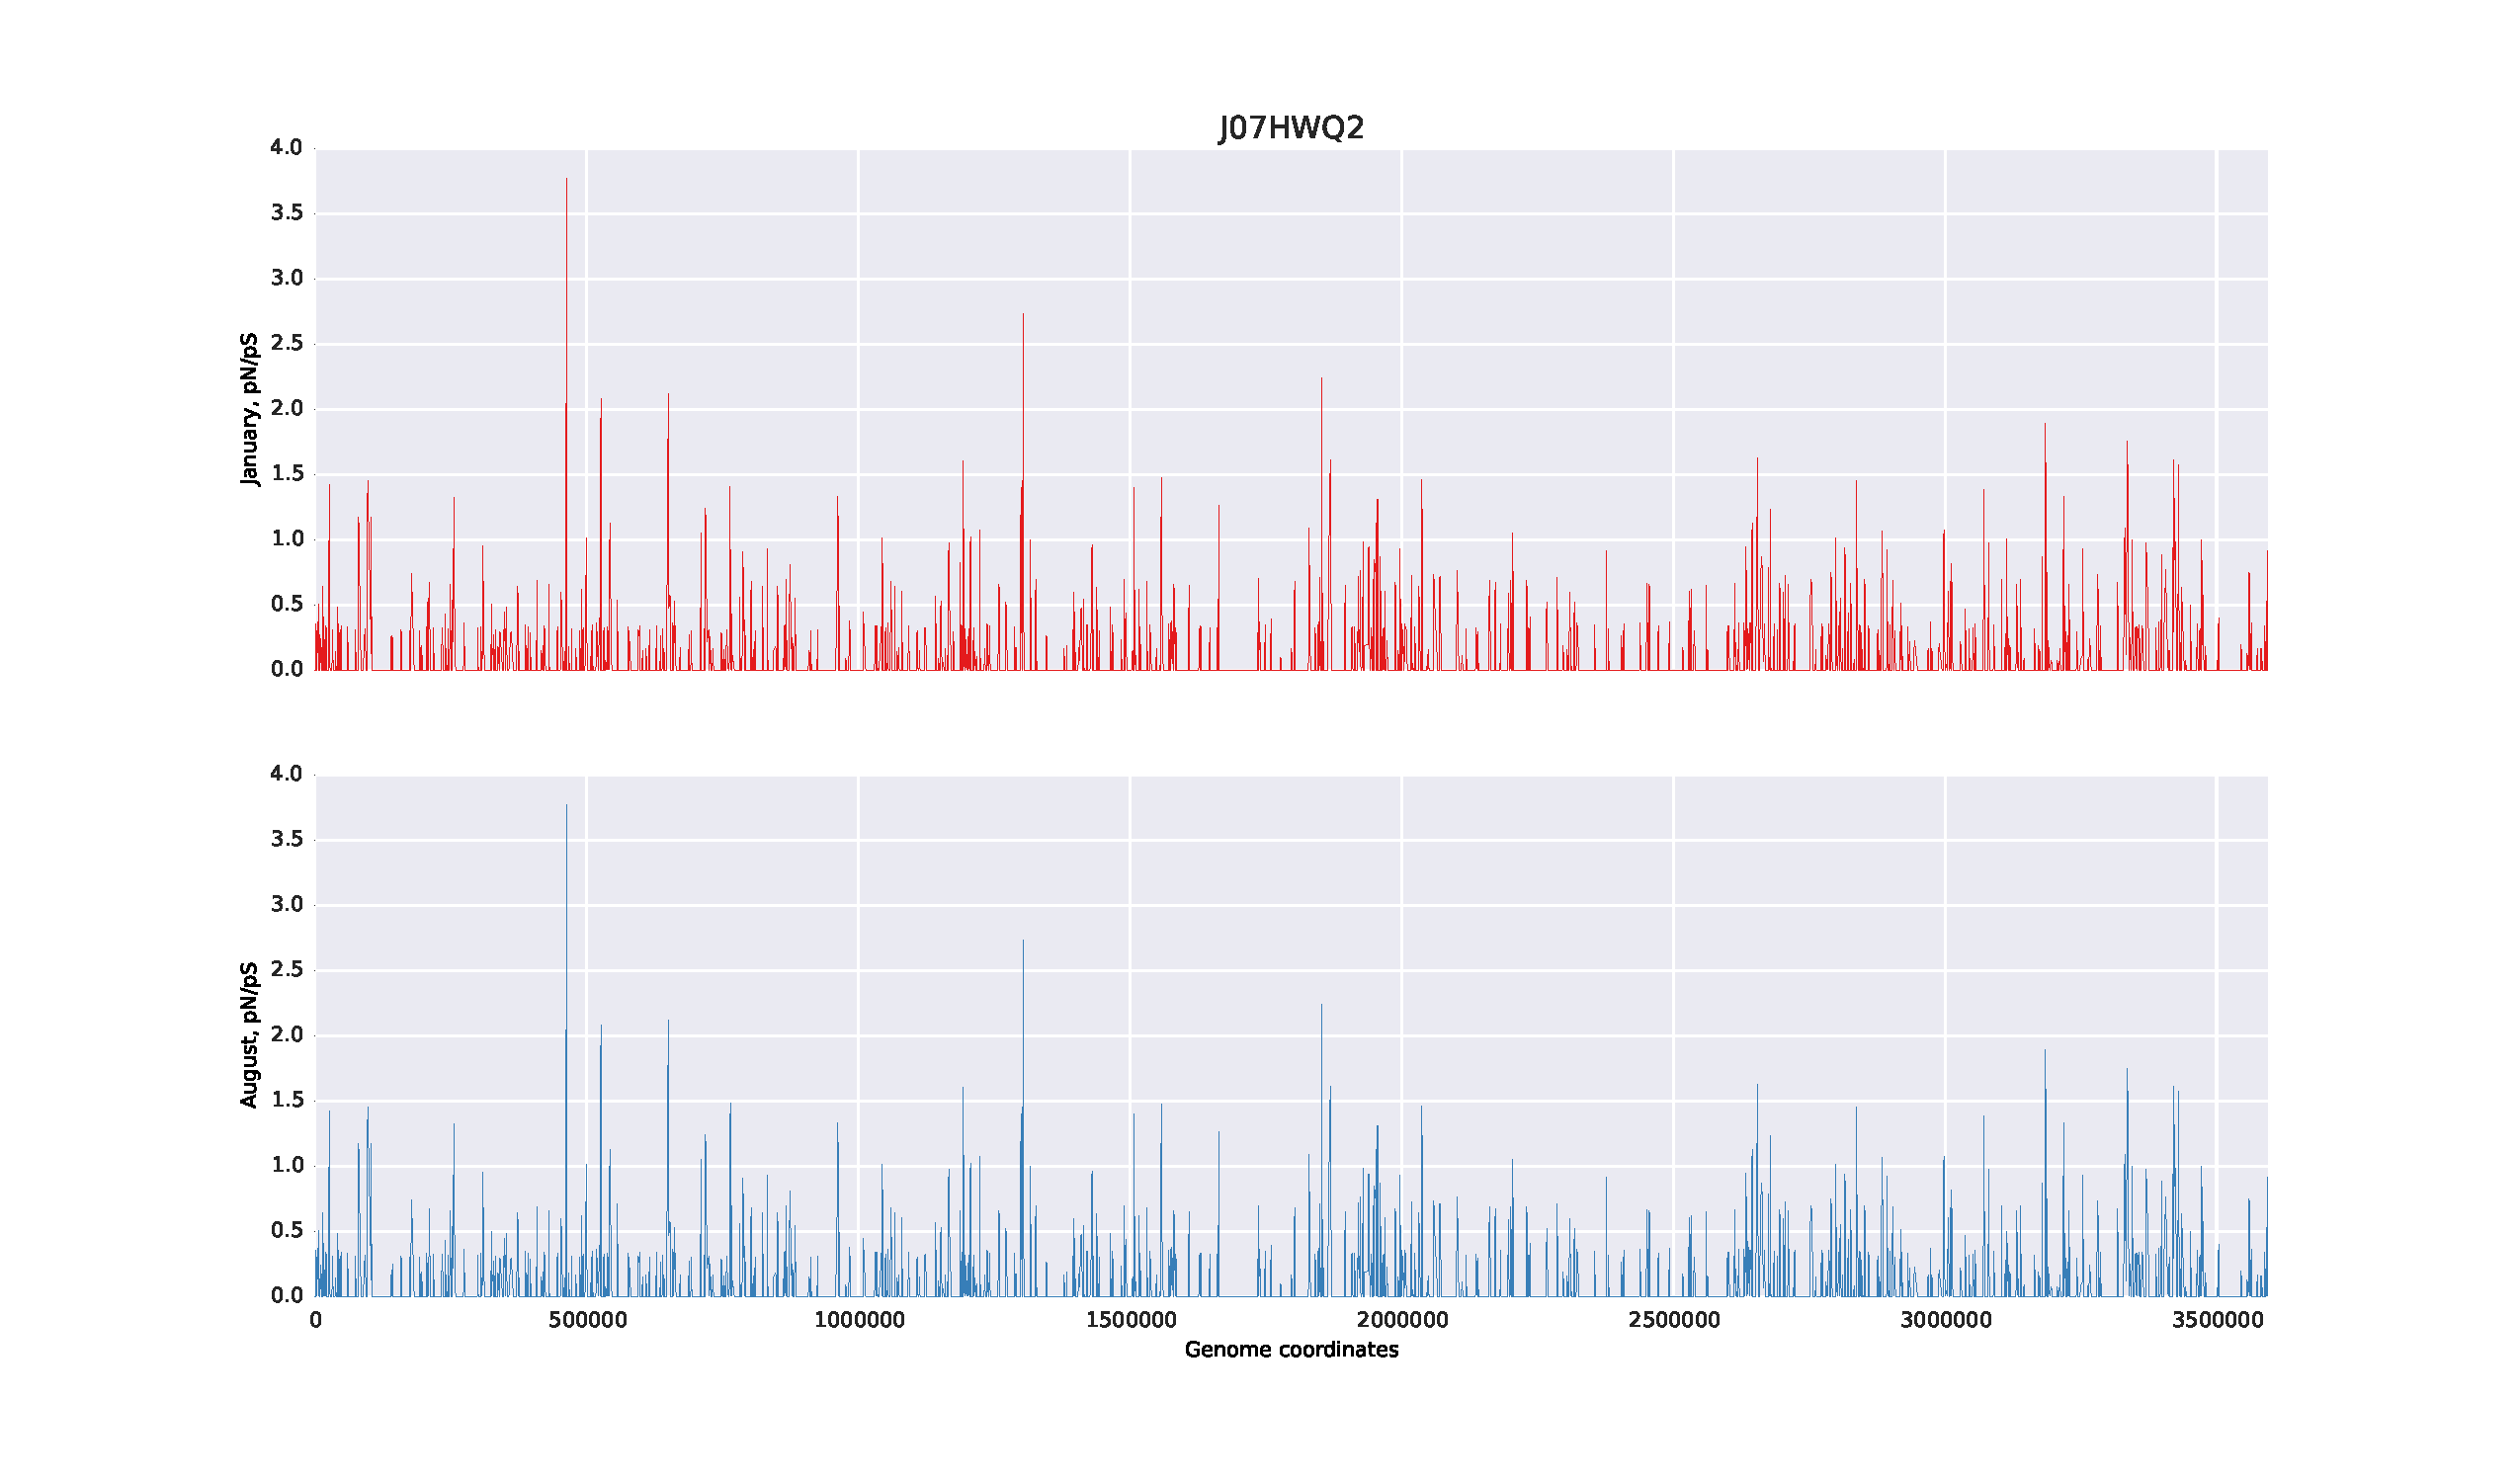
\includegraphics[width=\textwidth,height=\textheight,keepaspectratio]{Chapter5/Figures/pn_ps_plots/J07HWQ2_pNpS_density.pdf}
  \caption{pN/pS values for each gene in the J07HWQ2 genome. Top panel shows the values using the reads from the January samples. Bottom panel shows the values using the reads from the August sample}
  \label{J07HWQ2_pNpS}
\end{figure}

\begin{figure}[p]
  \centering
  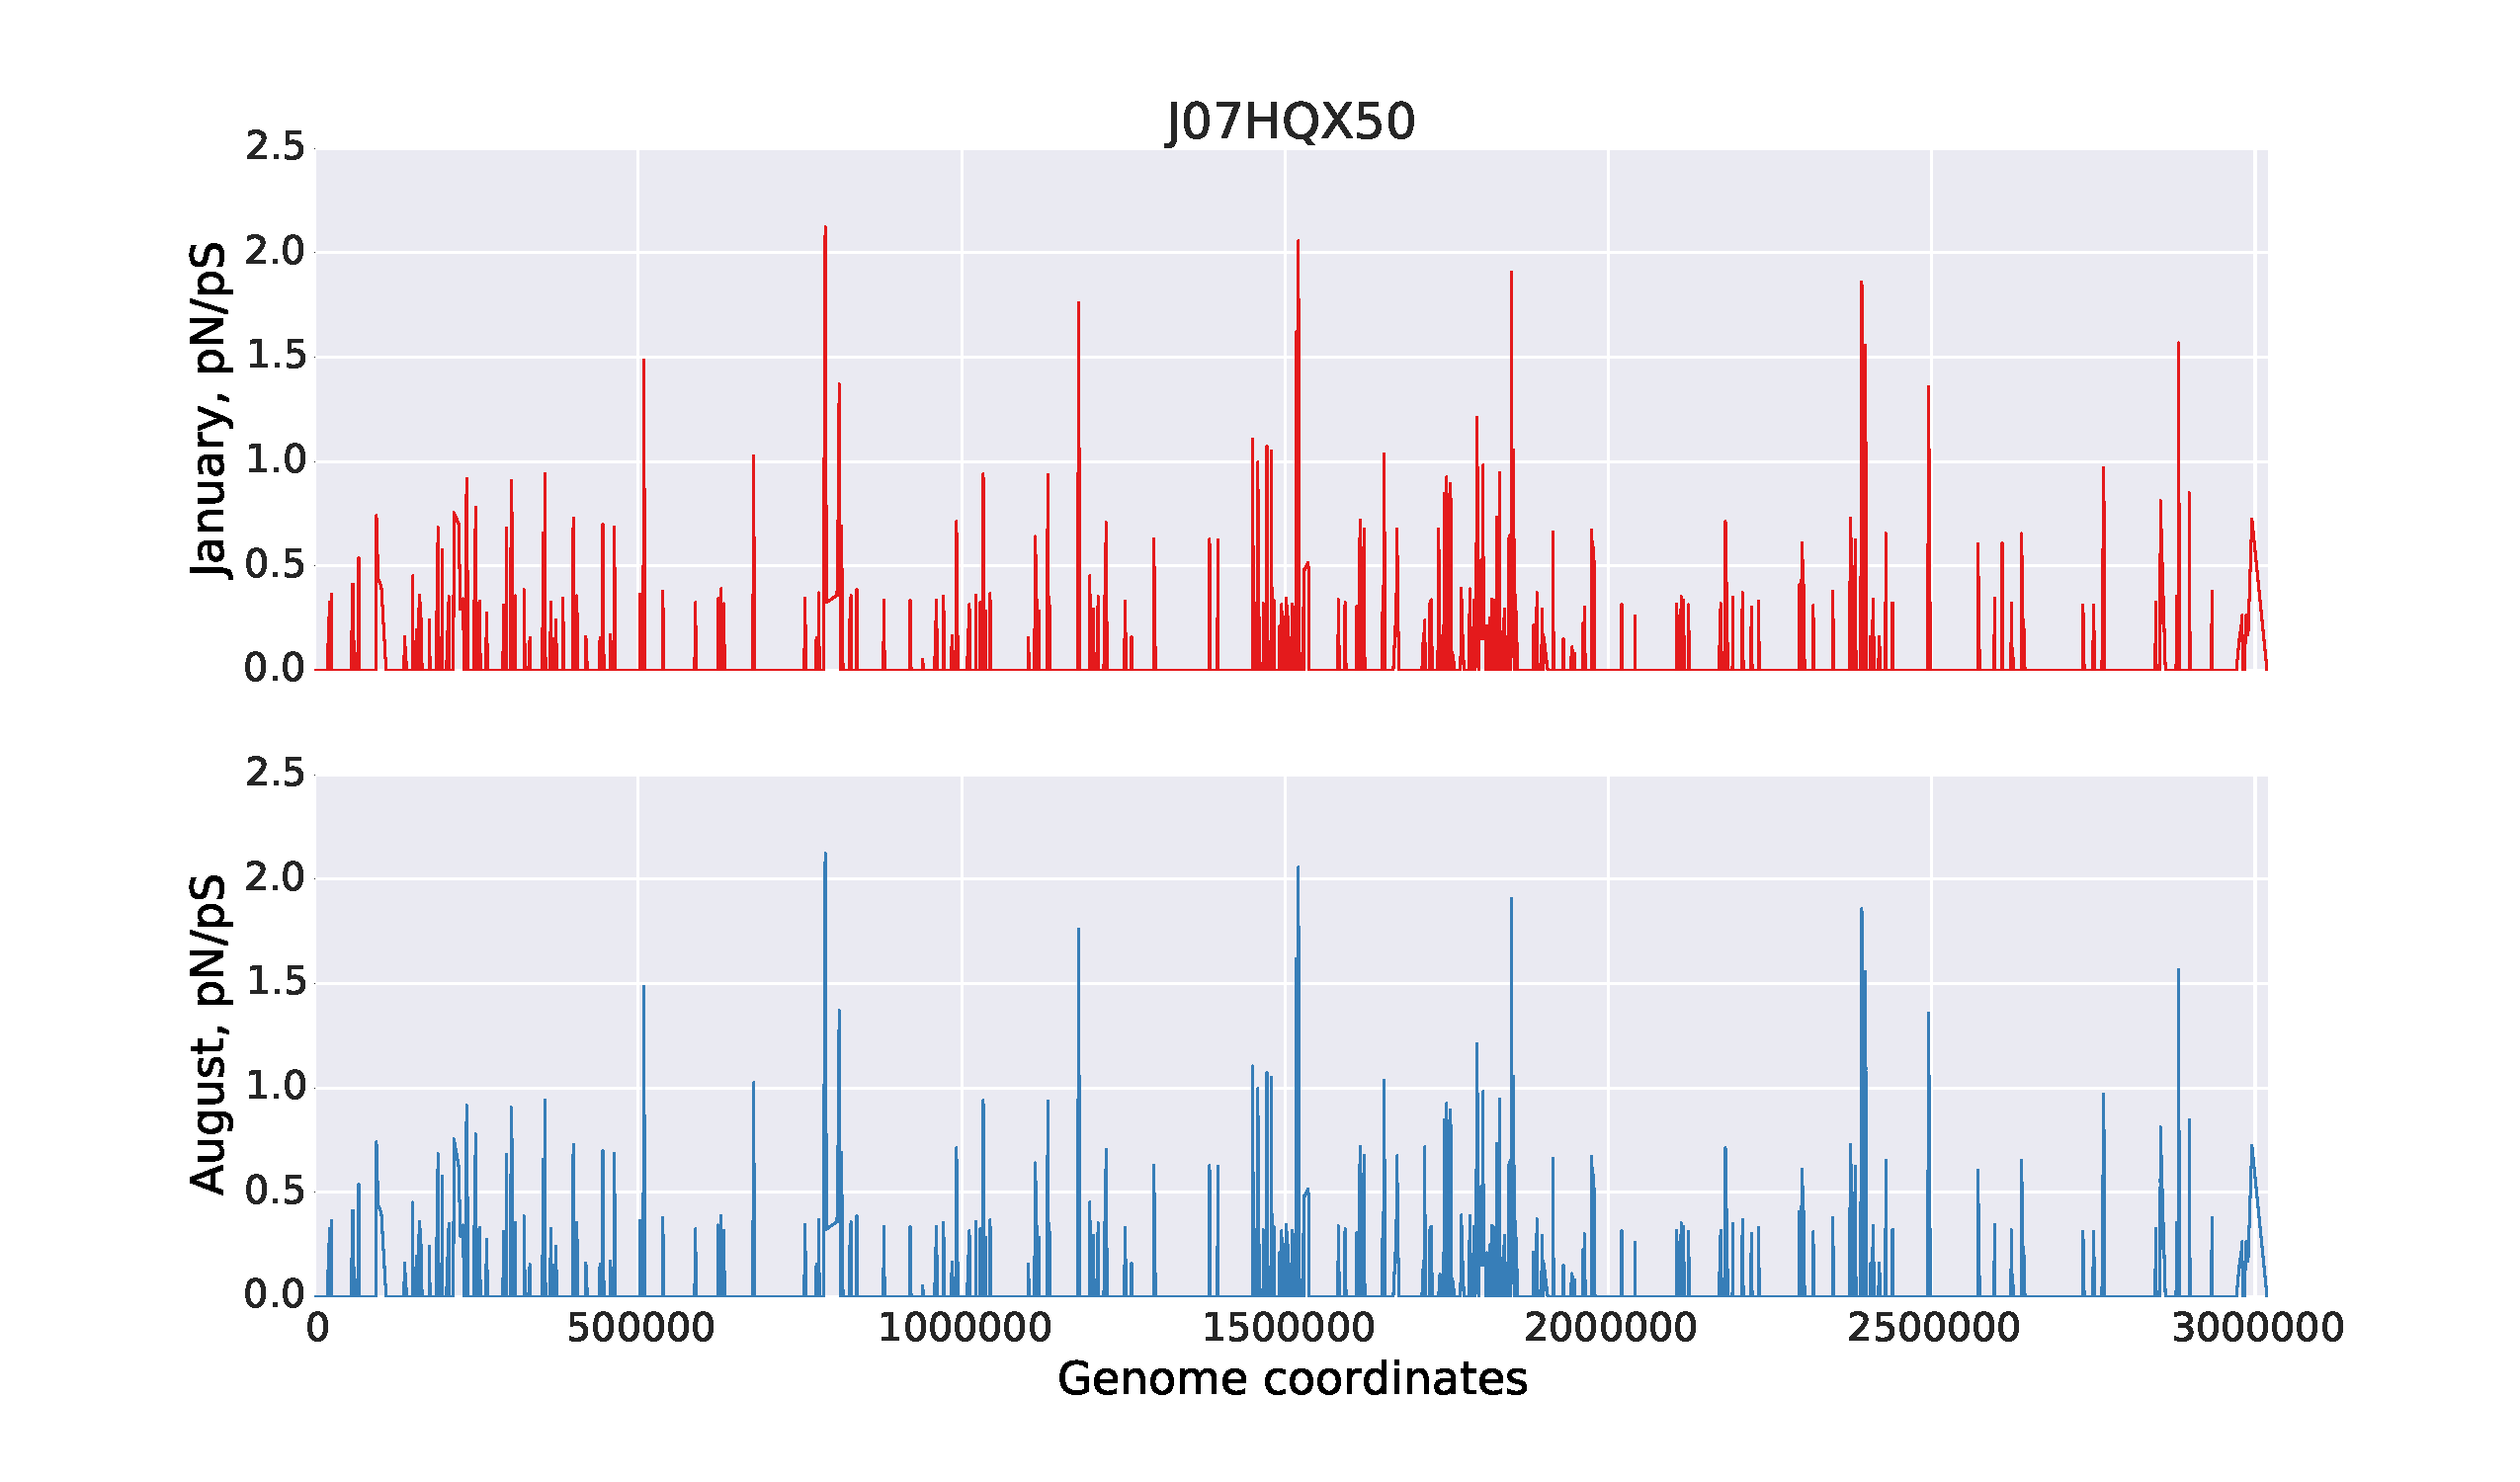
\includegraphics[width=\textwidth,height=\textheight,keepaspectratio]{Chapter5/Figures/pn_ps_plots/J07HQX50_pNpS_density.pdf}
  \caption{pN/pS values for each gene in the J07HQX50 genome. Top panel shows the values using the reads from the January samples. Bottom panel shows the values using the reads from the August sample}
  \label{J07HQX50_pNpS}
\end{figure}

\begin{figure}[p]
  \centering
  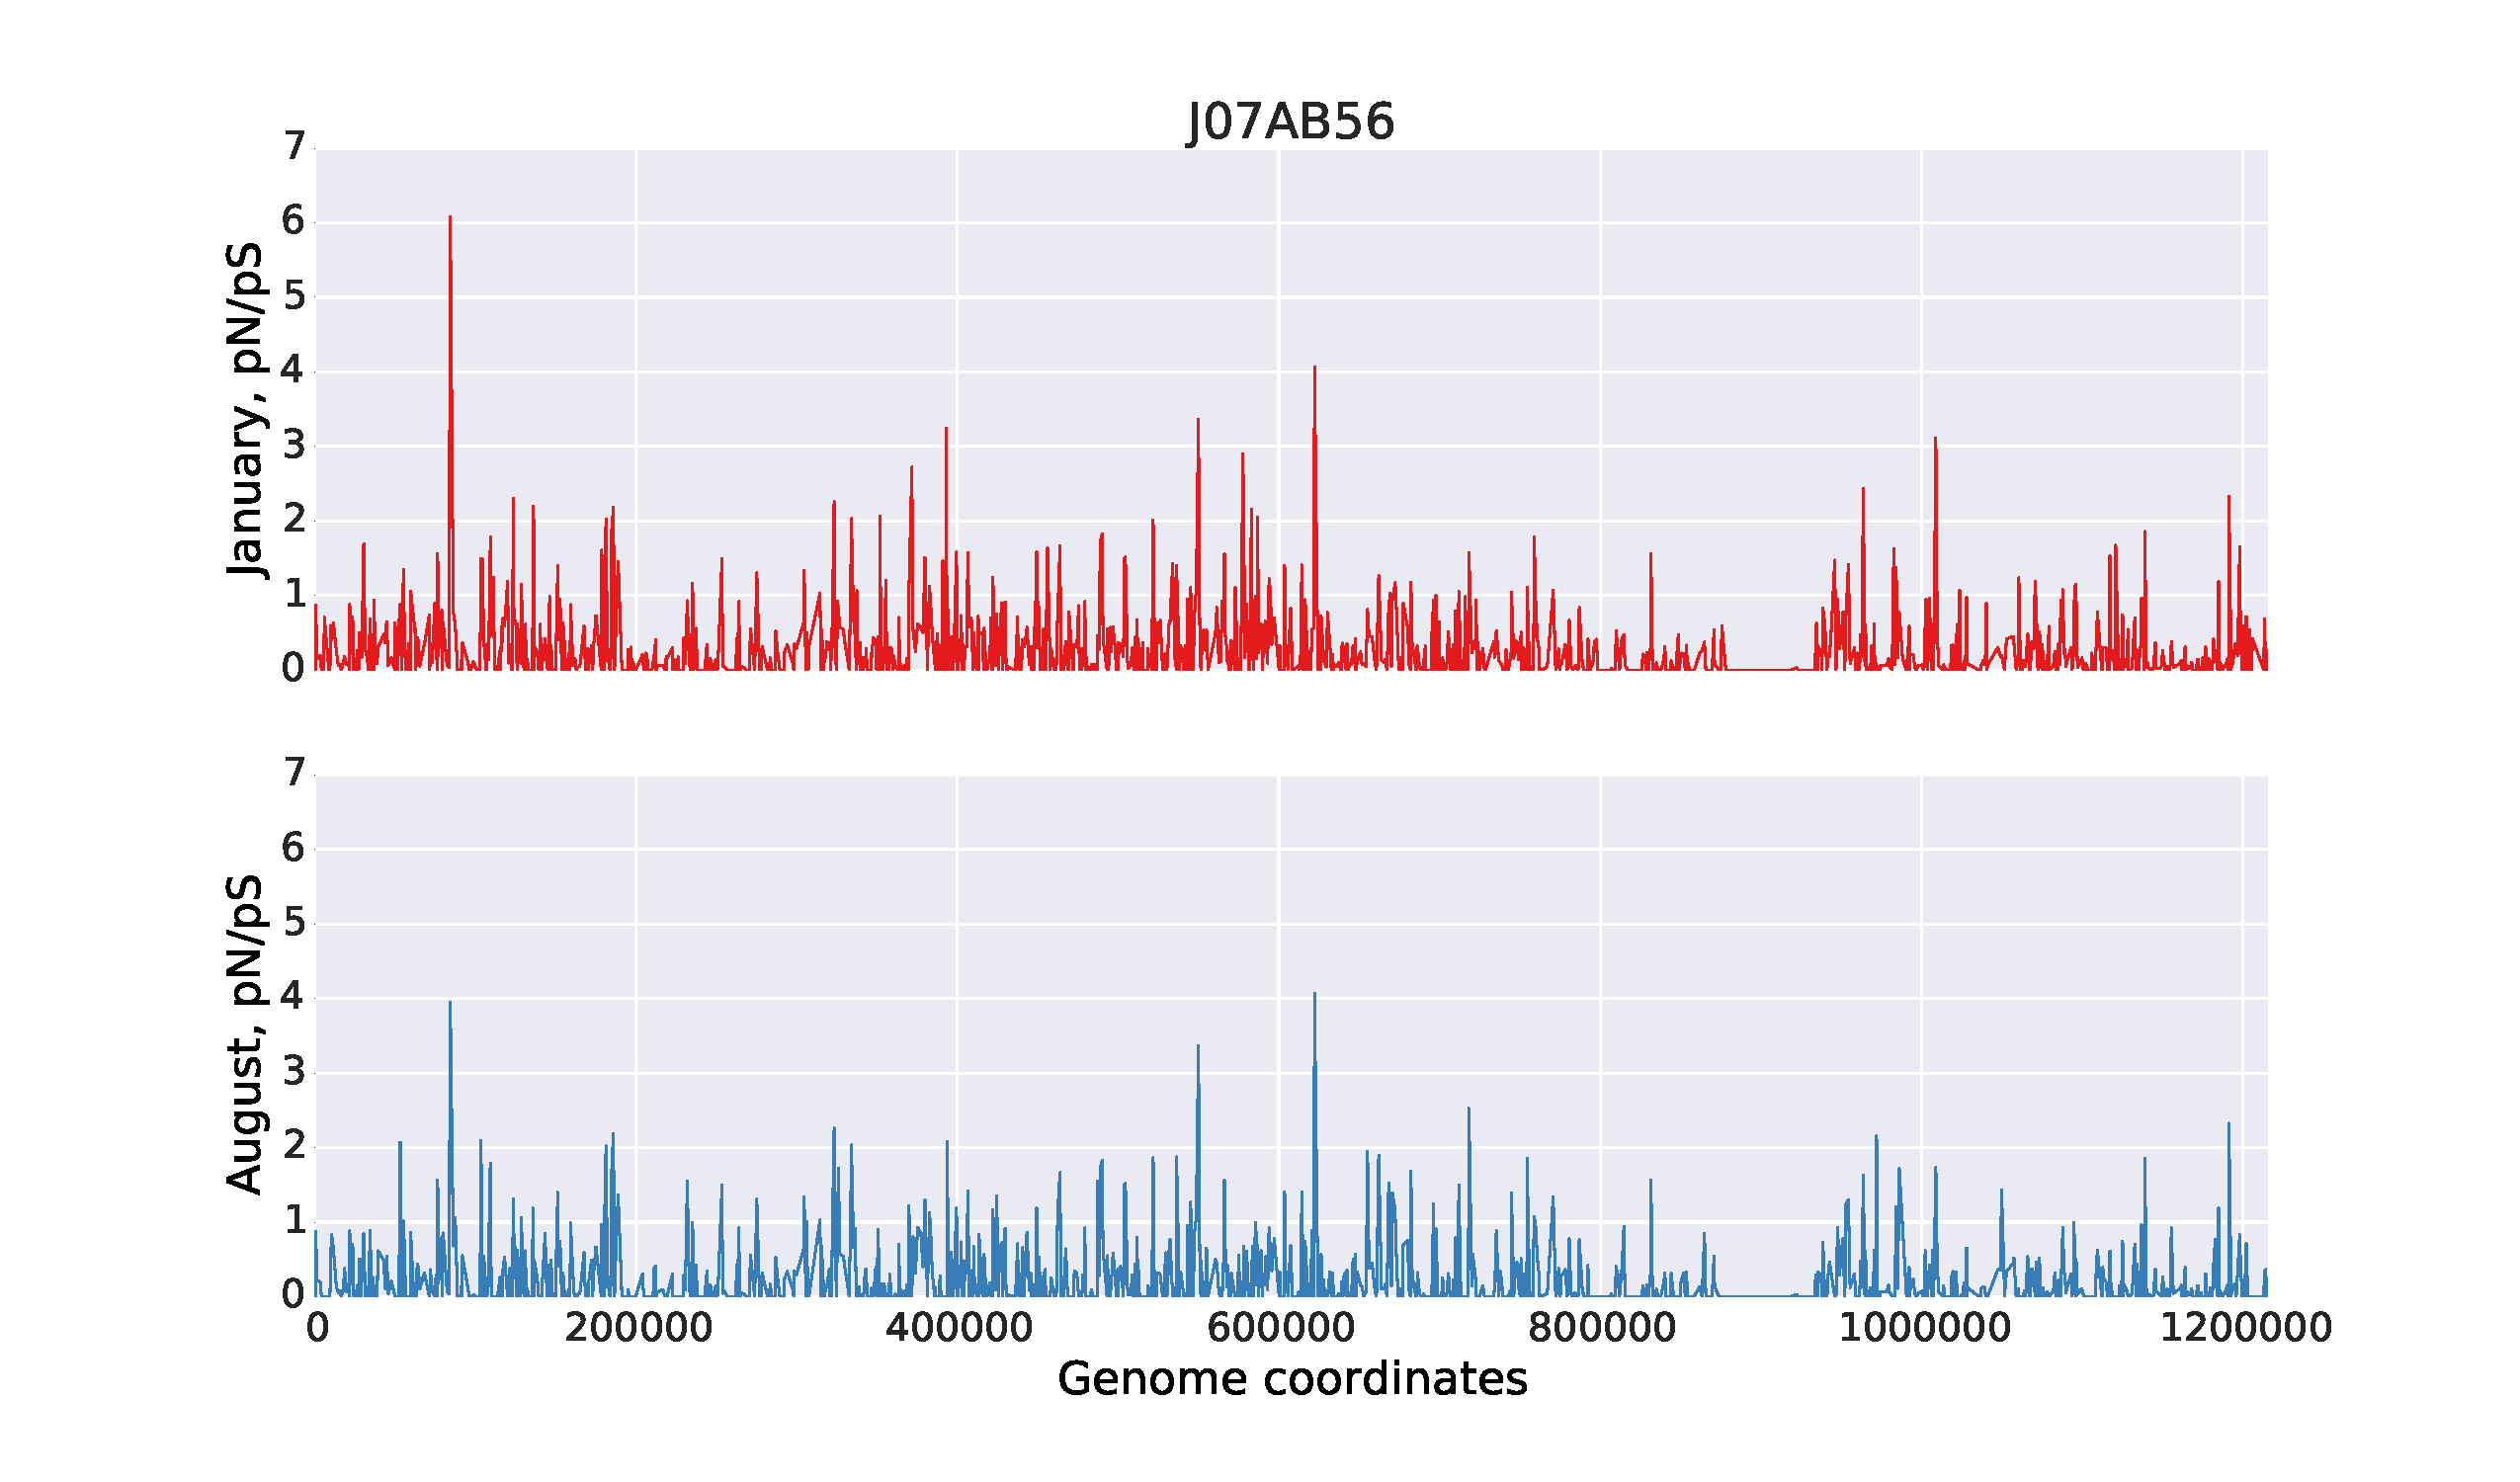
\includegraphics[width=\textwidth,height=\textheight,keepaspectratio]{Chapter5/Figures/pn_ps_plots/J07AB56_pNpS_density.pdf}
  \caption{pN/pS values for each gene in the J07AB56 genome. Top panel shows the values using the reads from the January samples. Bottom panel shows the values using the reads from the August sample}
  \label{J07AB56_pNpS}
\end{figure}

\begin{figure}[p]
  \centering
  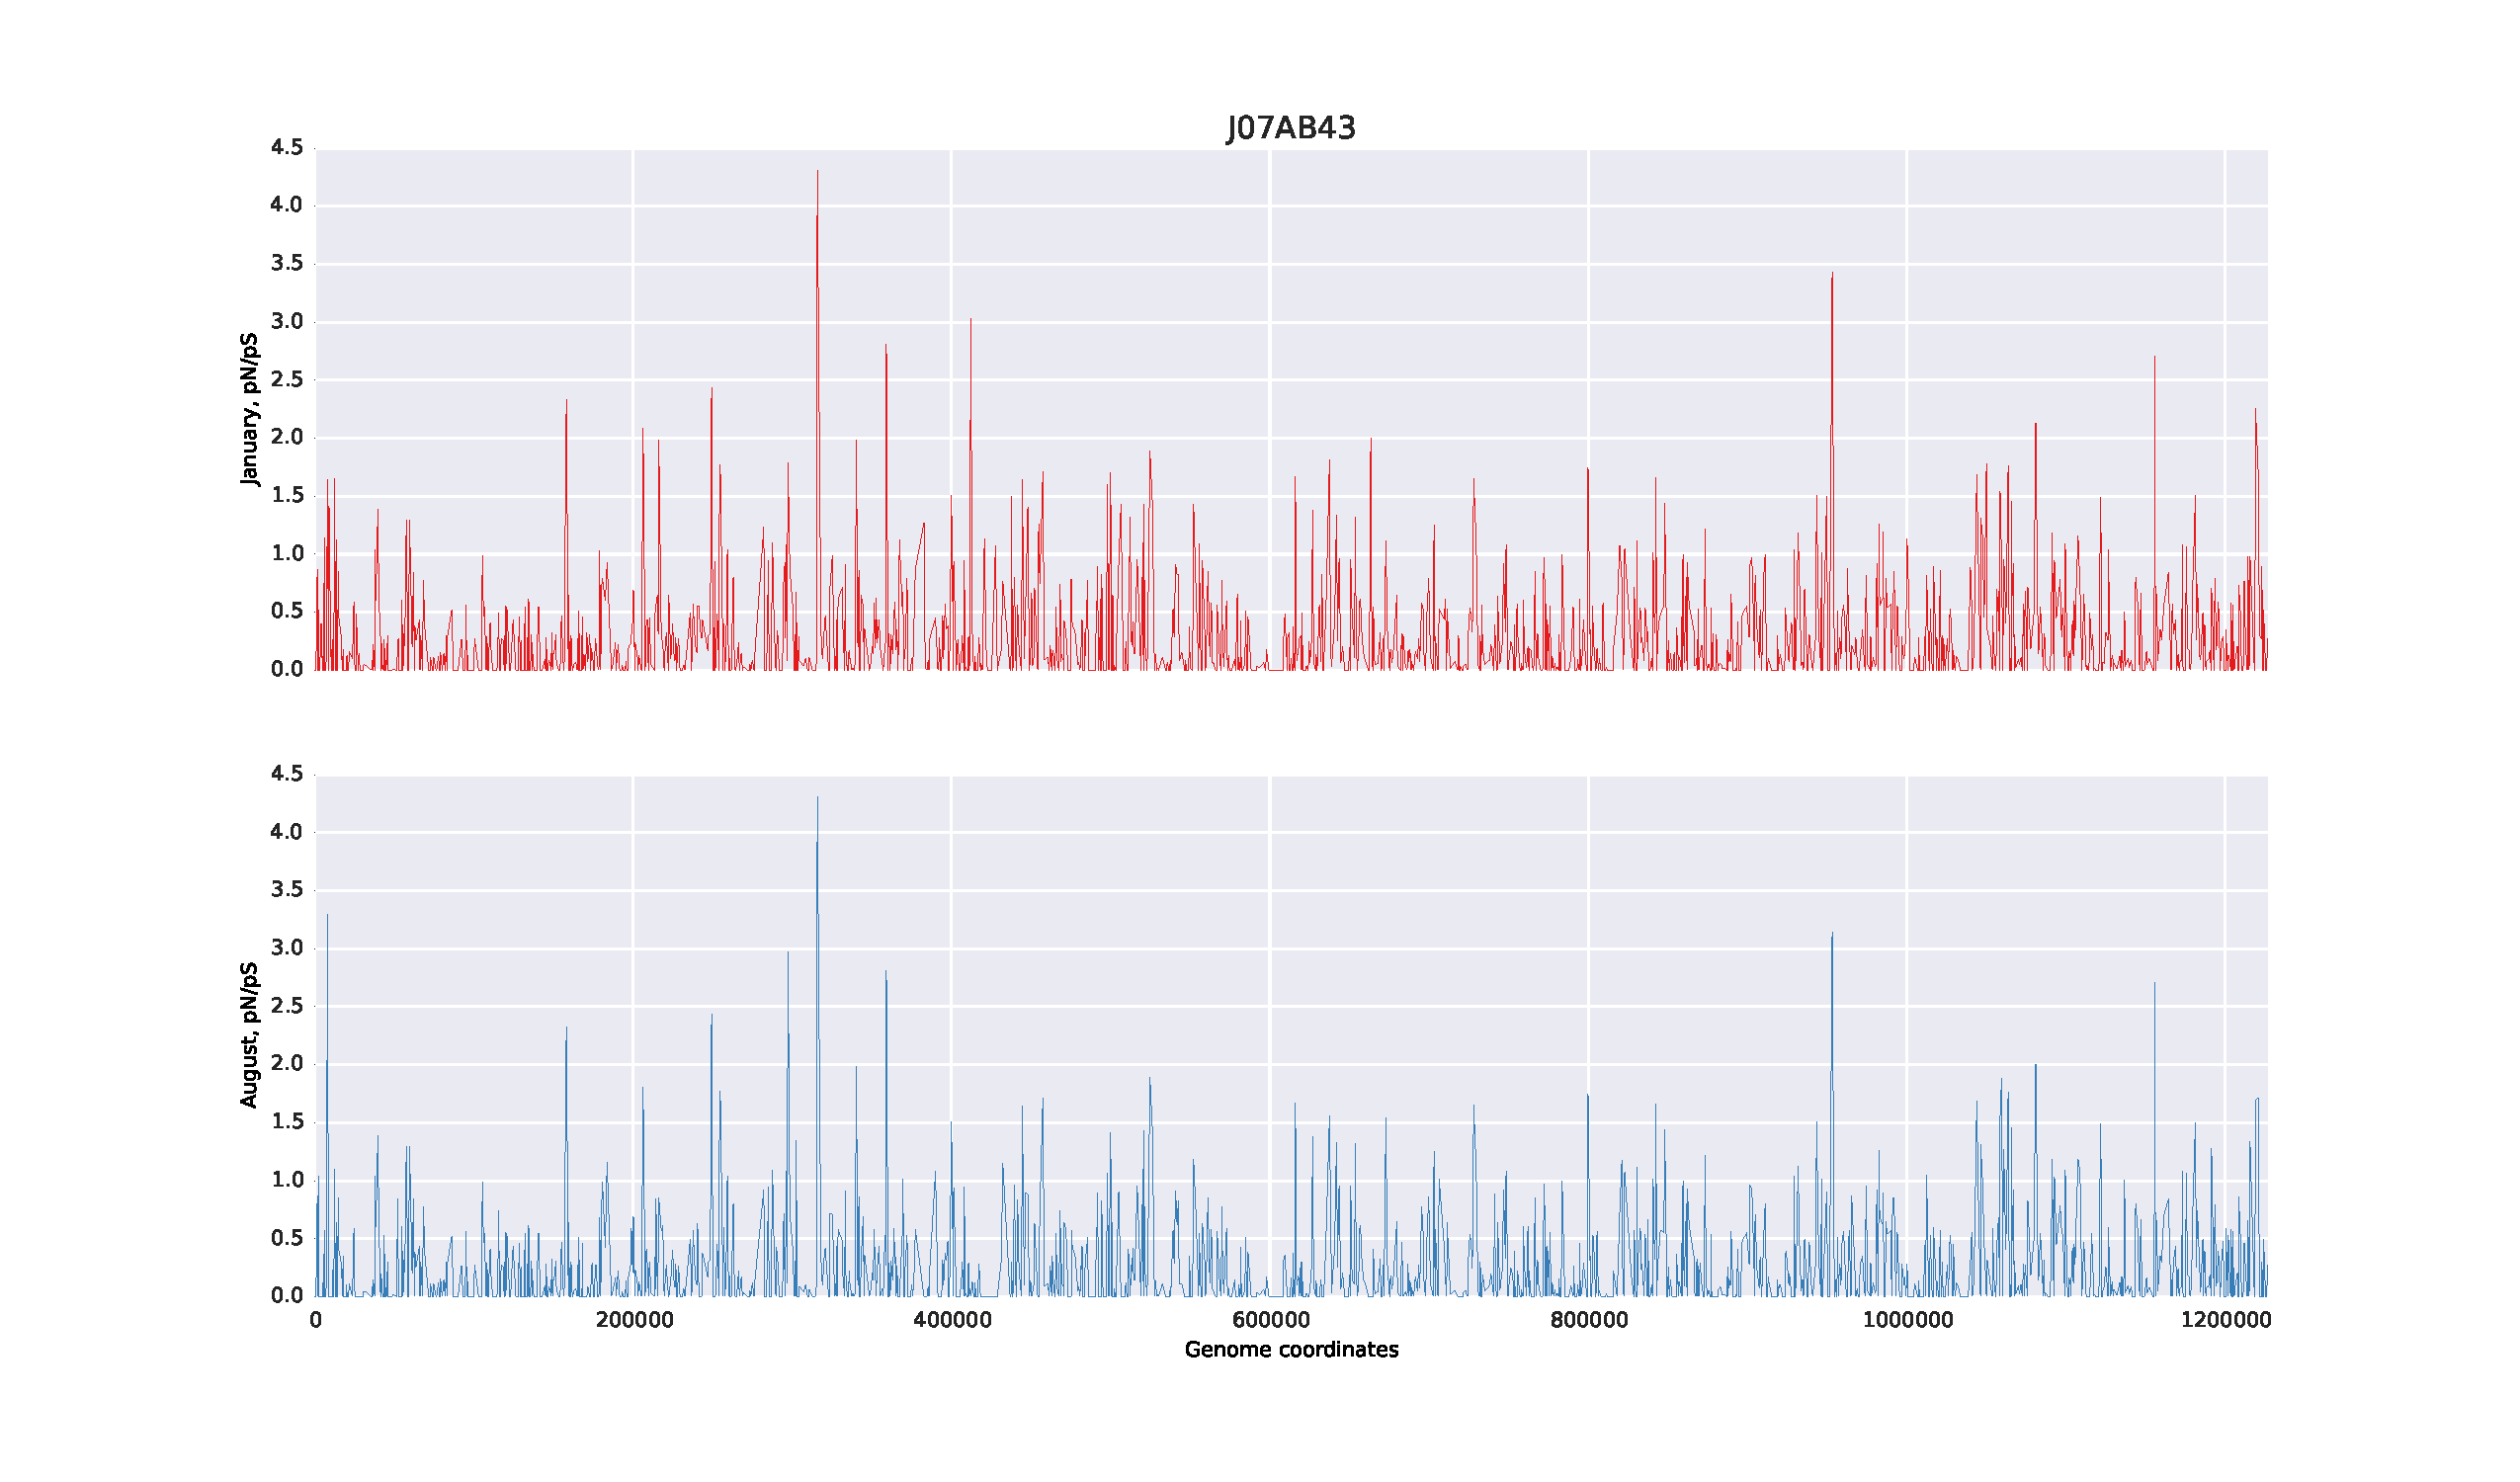
\includegraphics[width=\textwidth,height=\textheight,keepaspectratio]{Chapter5/Figures/pn_ps_plots/J07AB43_pNpS_density.pdf}
  \caption{pN/pS values for each gene in the J07AB56 genome. Top panel shows the values using the reads from the January samples. Bottom panel shows the values using the reads from the August sample}
  \label{J07AB43_pNpS}
\end{figure}

\begin{figure}[p]
  \centering
  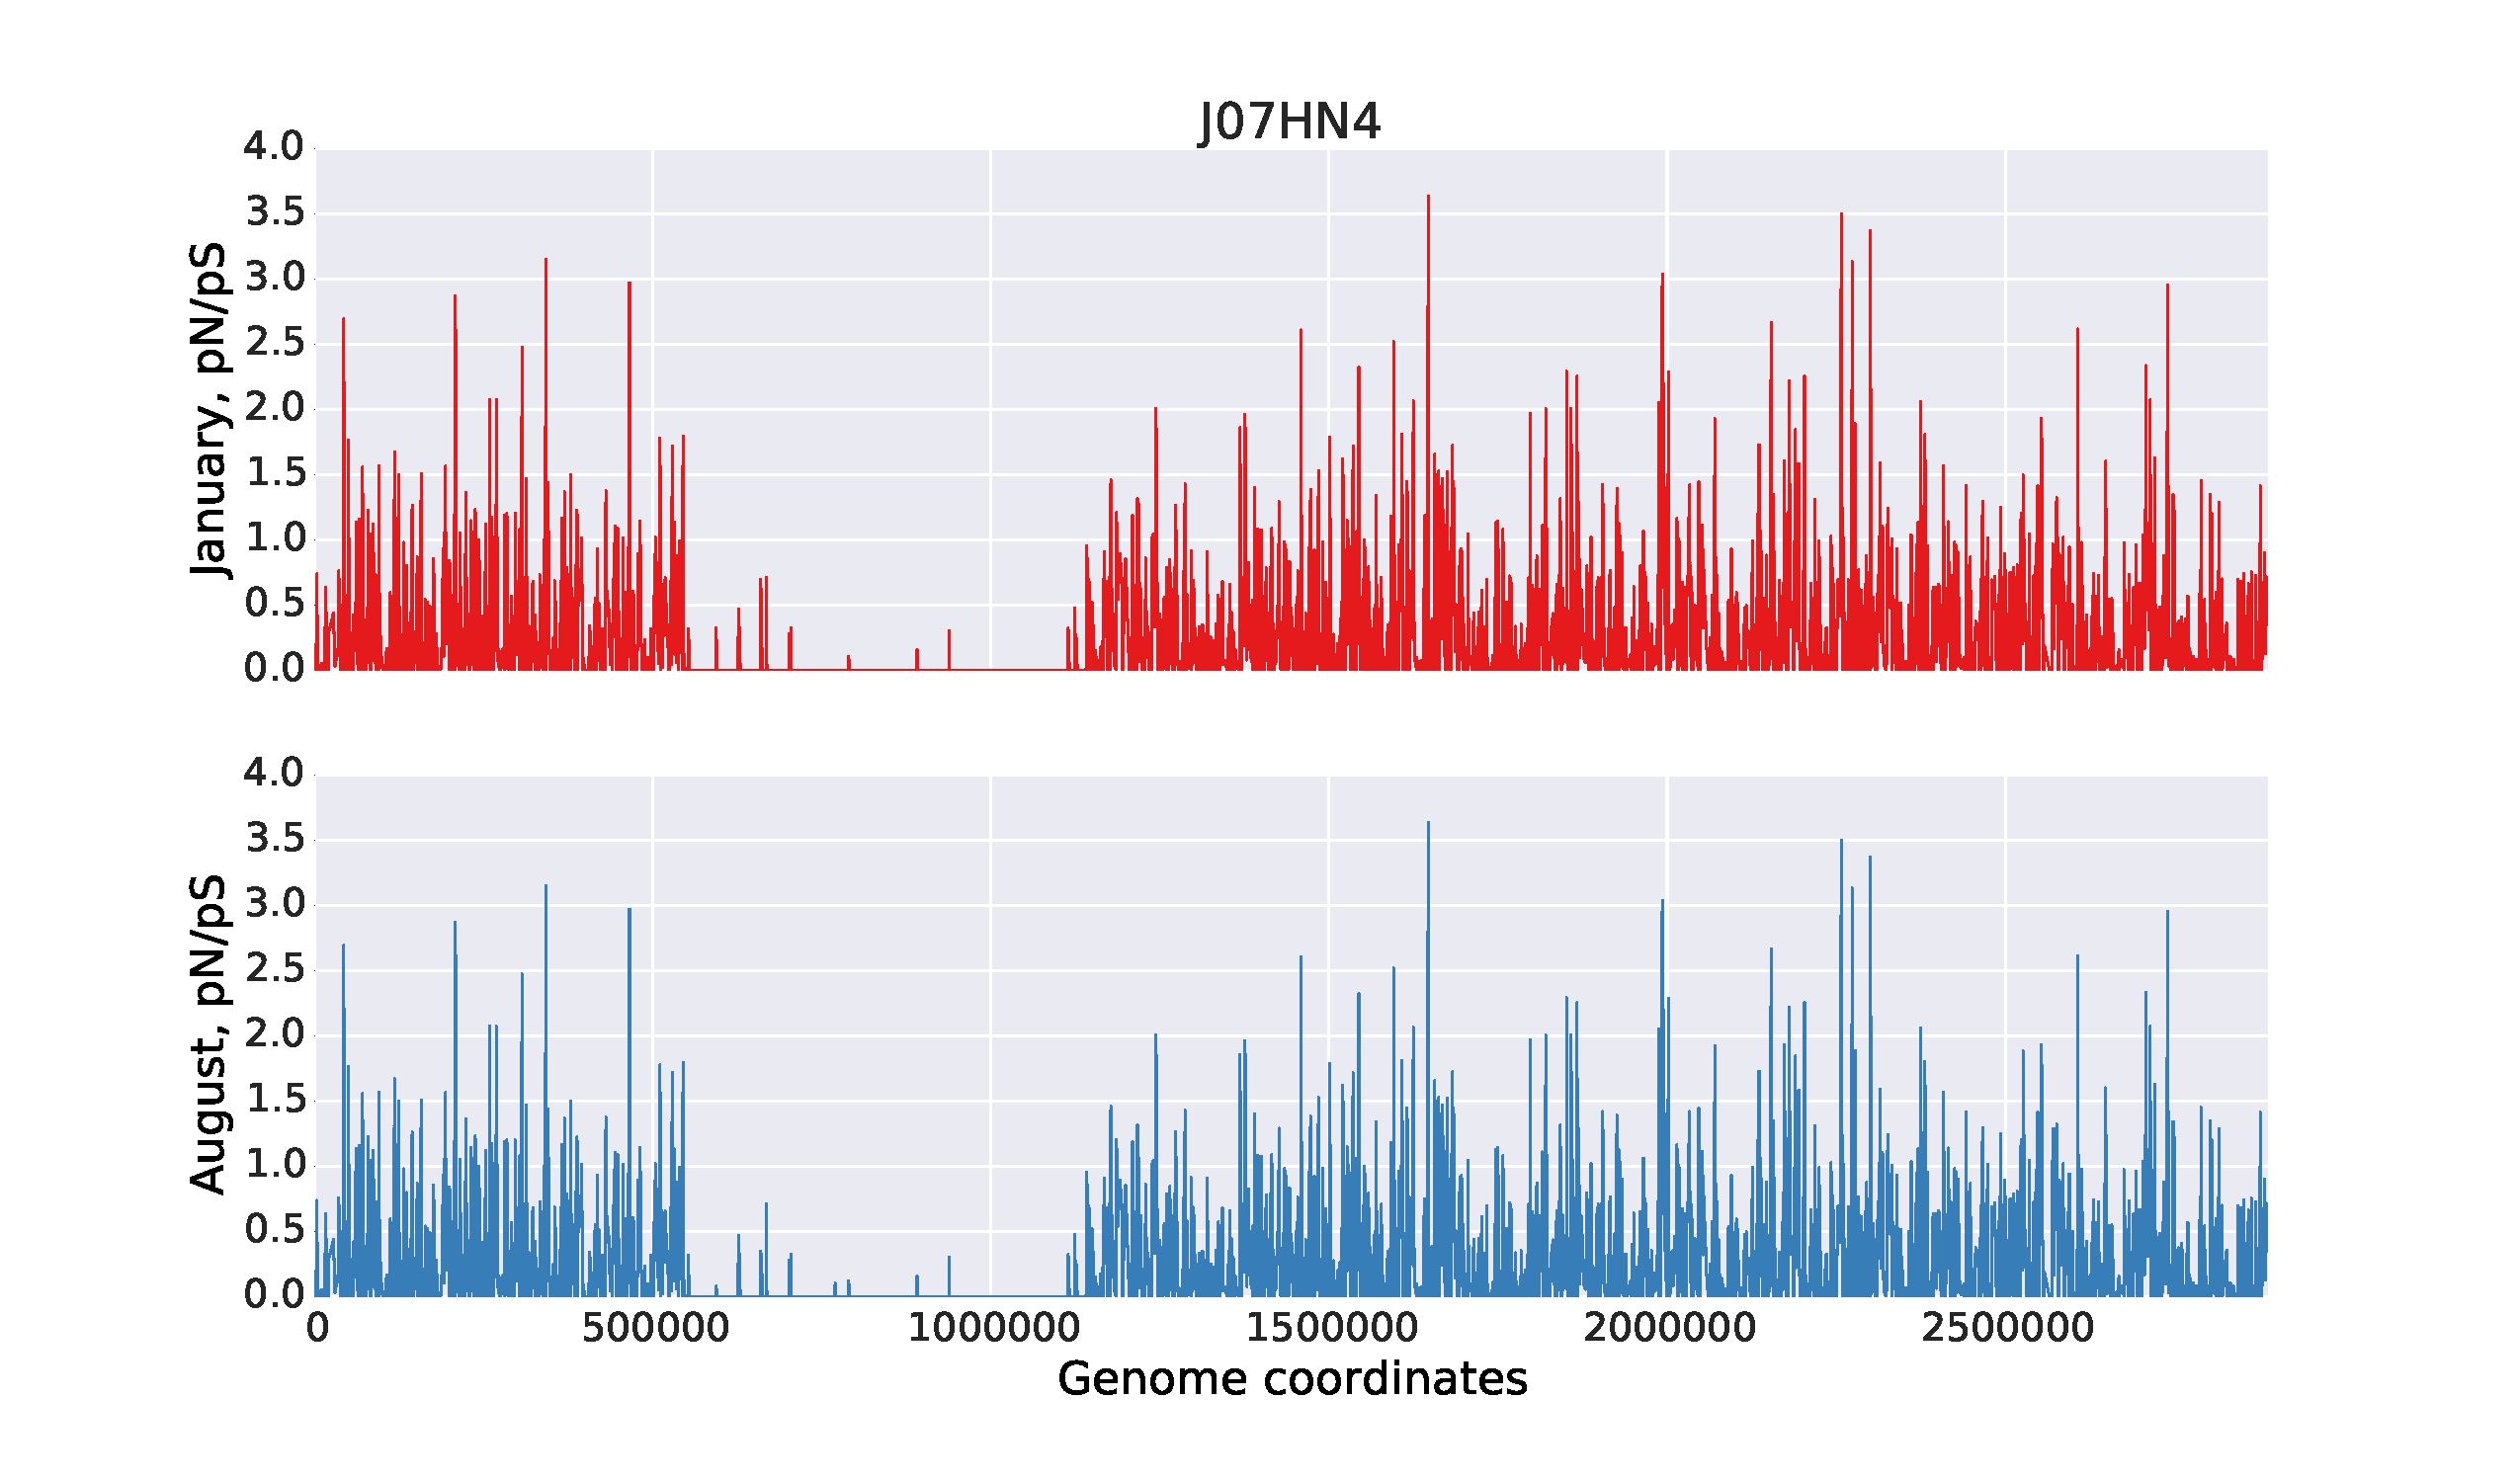
\includegraphics[width=\textwidth,height=\textheight,keepaspectratio]{Chapter5/Figures/pn_ps_plots/J07HN4_pNpS_density.pdf}
  \caption{pN/pS values for each gene in the J07HN4 genome. Top panel shows the values using the reads from the January samples. Bottom panel shows the values using the reads from the August sample}
  \label{J07HN4_pNpS}
\end{figure}

\begin{figure}[p]
  \centering
  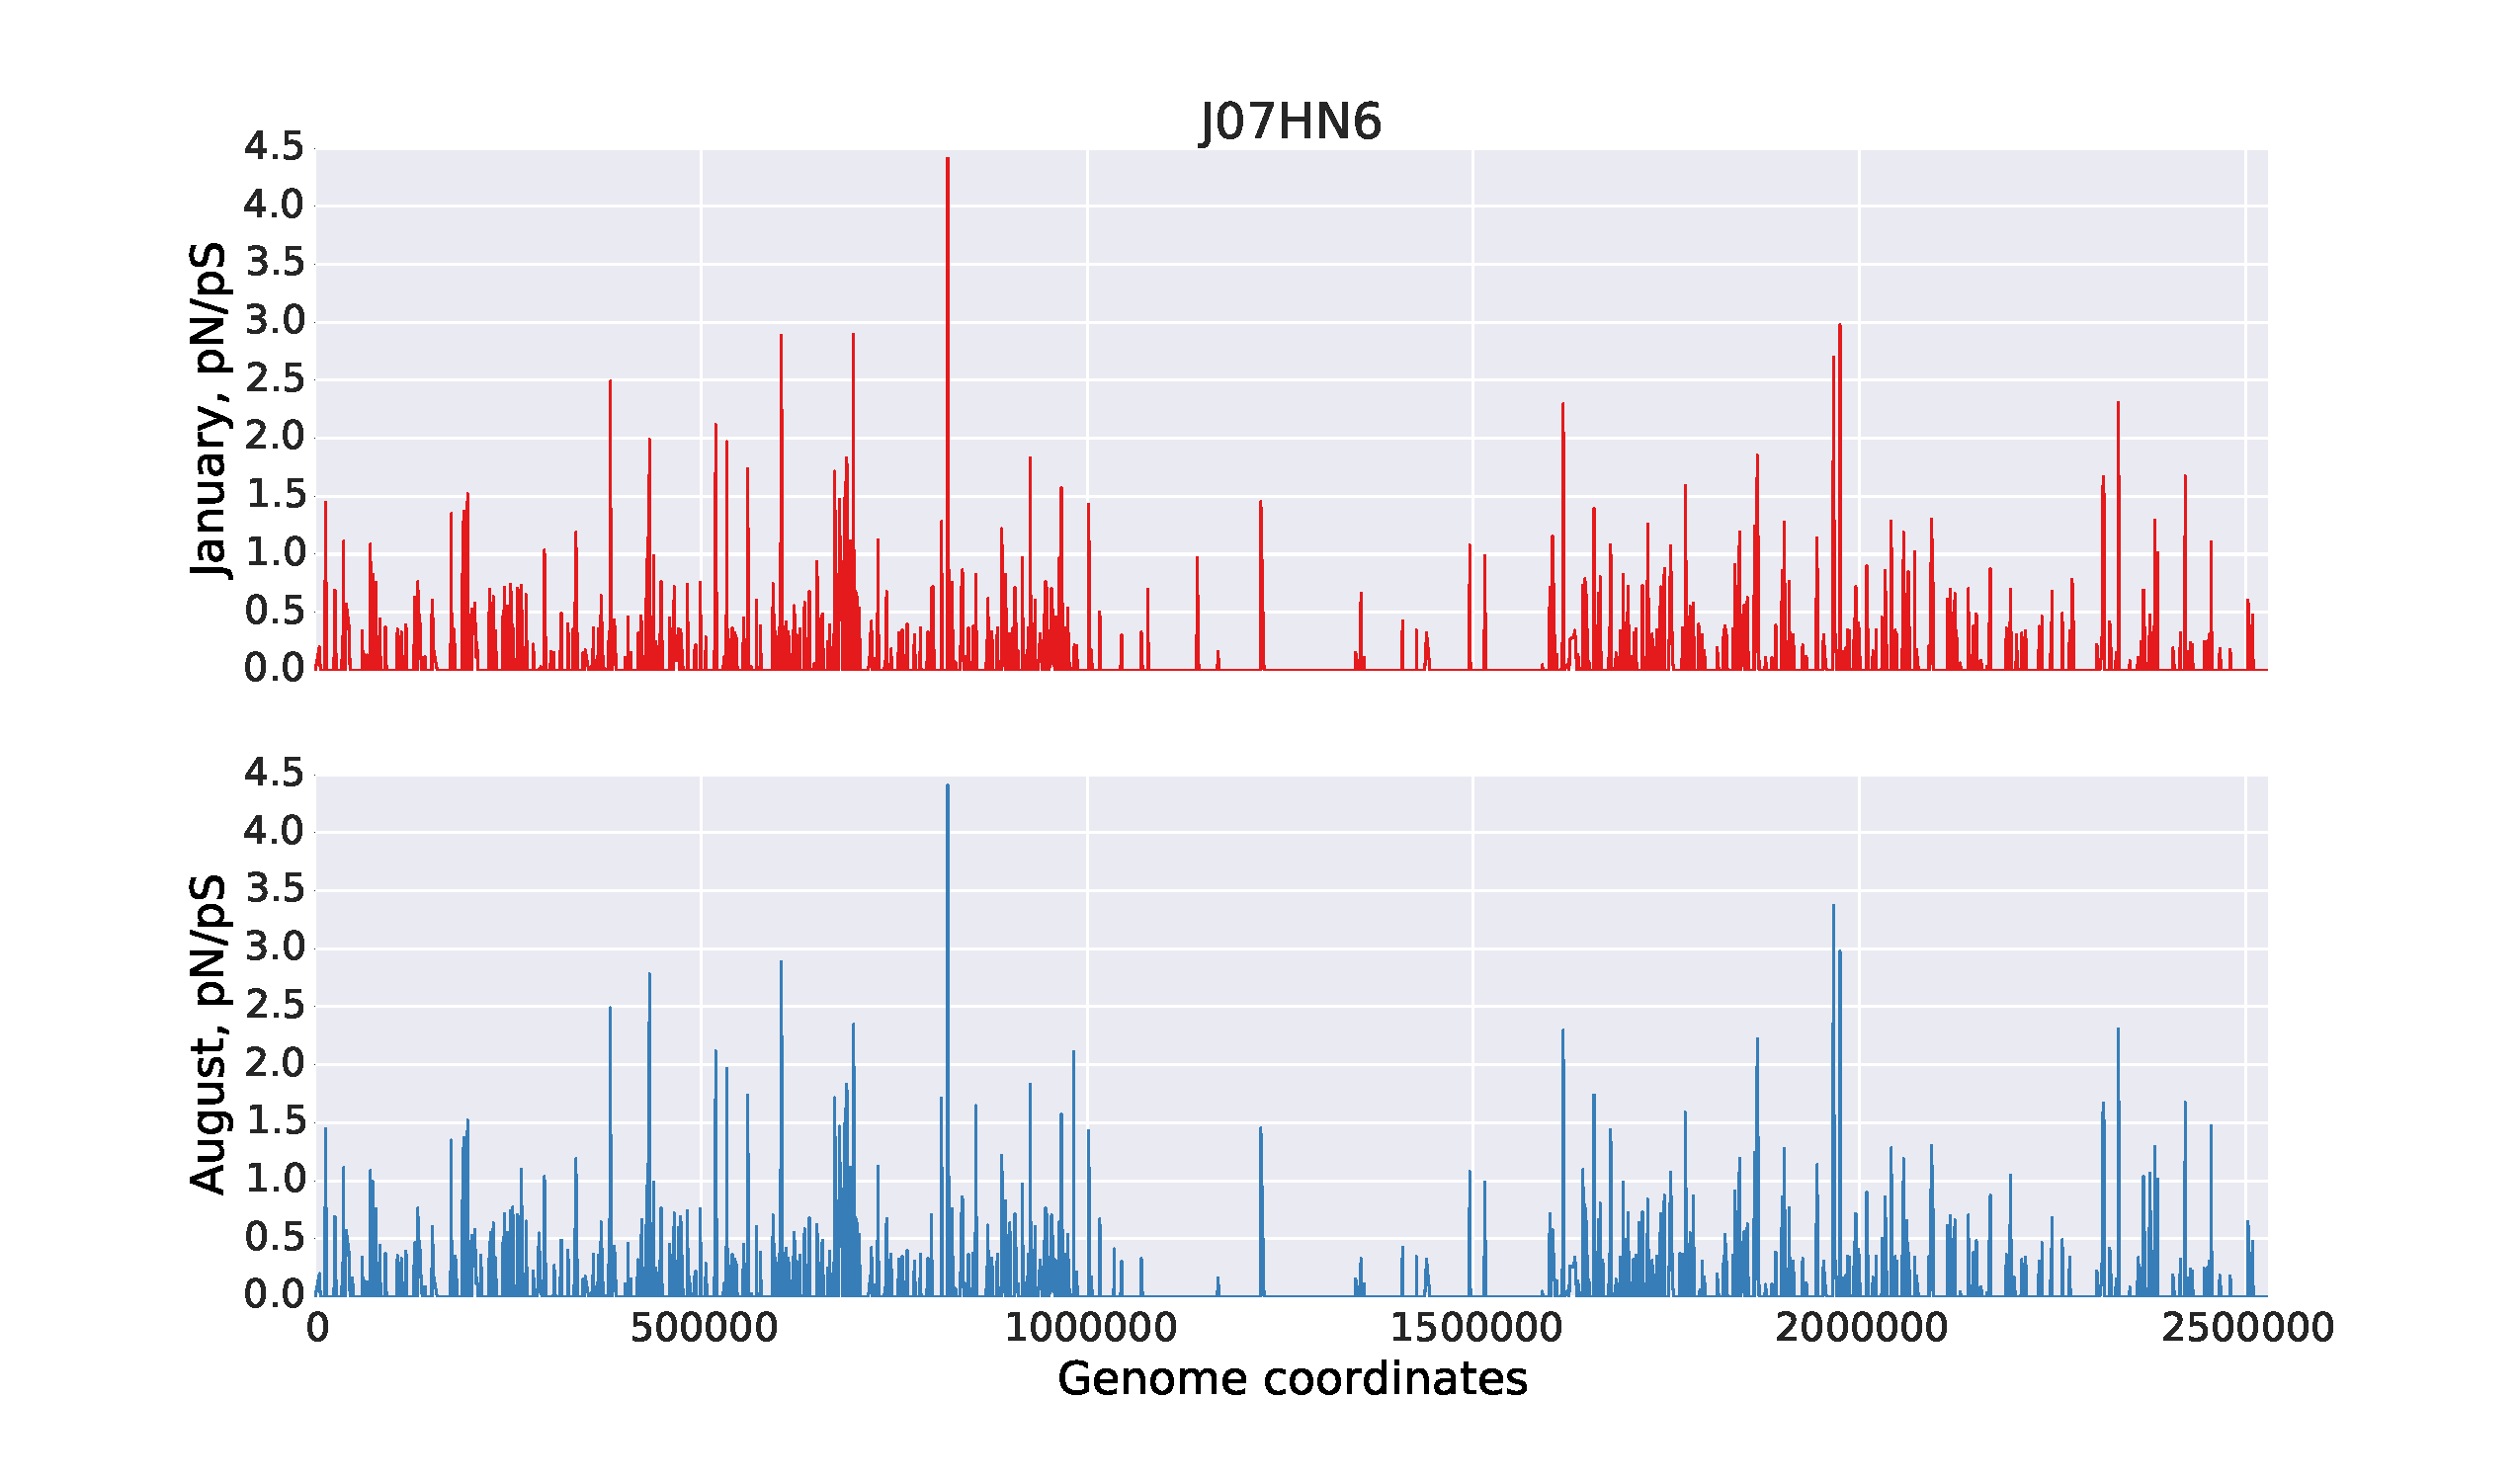
\includegraphics[width=\textwidth,height=\textheight,keepaspectratio]{Chapter5/Figures/pn_ps_plots/J07HN6_pNpS_density.pdf}
  \caption{pN/pS values for each gene in the J07HN6 genome. Top panel shows the values using the reads from the January samples. Bottom panel shows the values using the reads from the August sample}
  \label{J07HN6_pNpS}
\end{figure}

\begin{figure}[p]
  \centering
  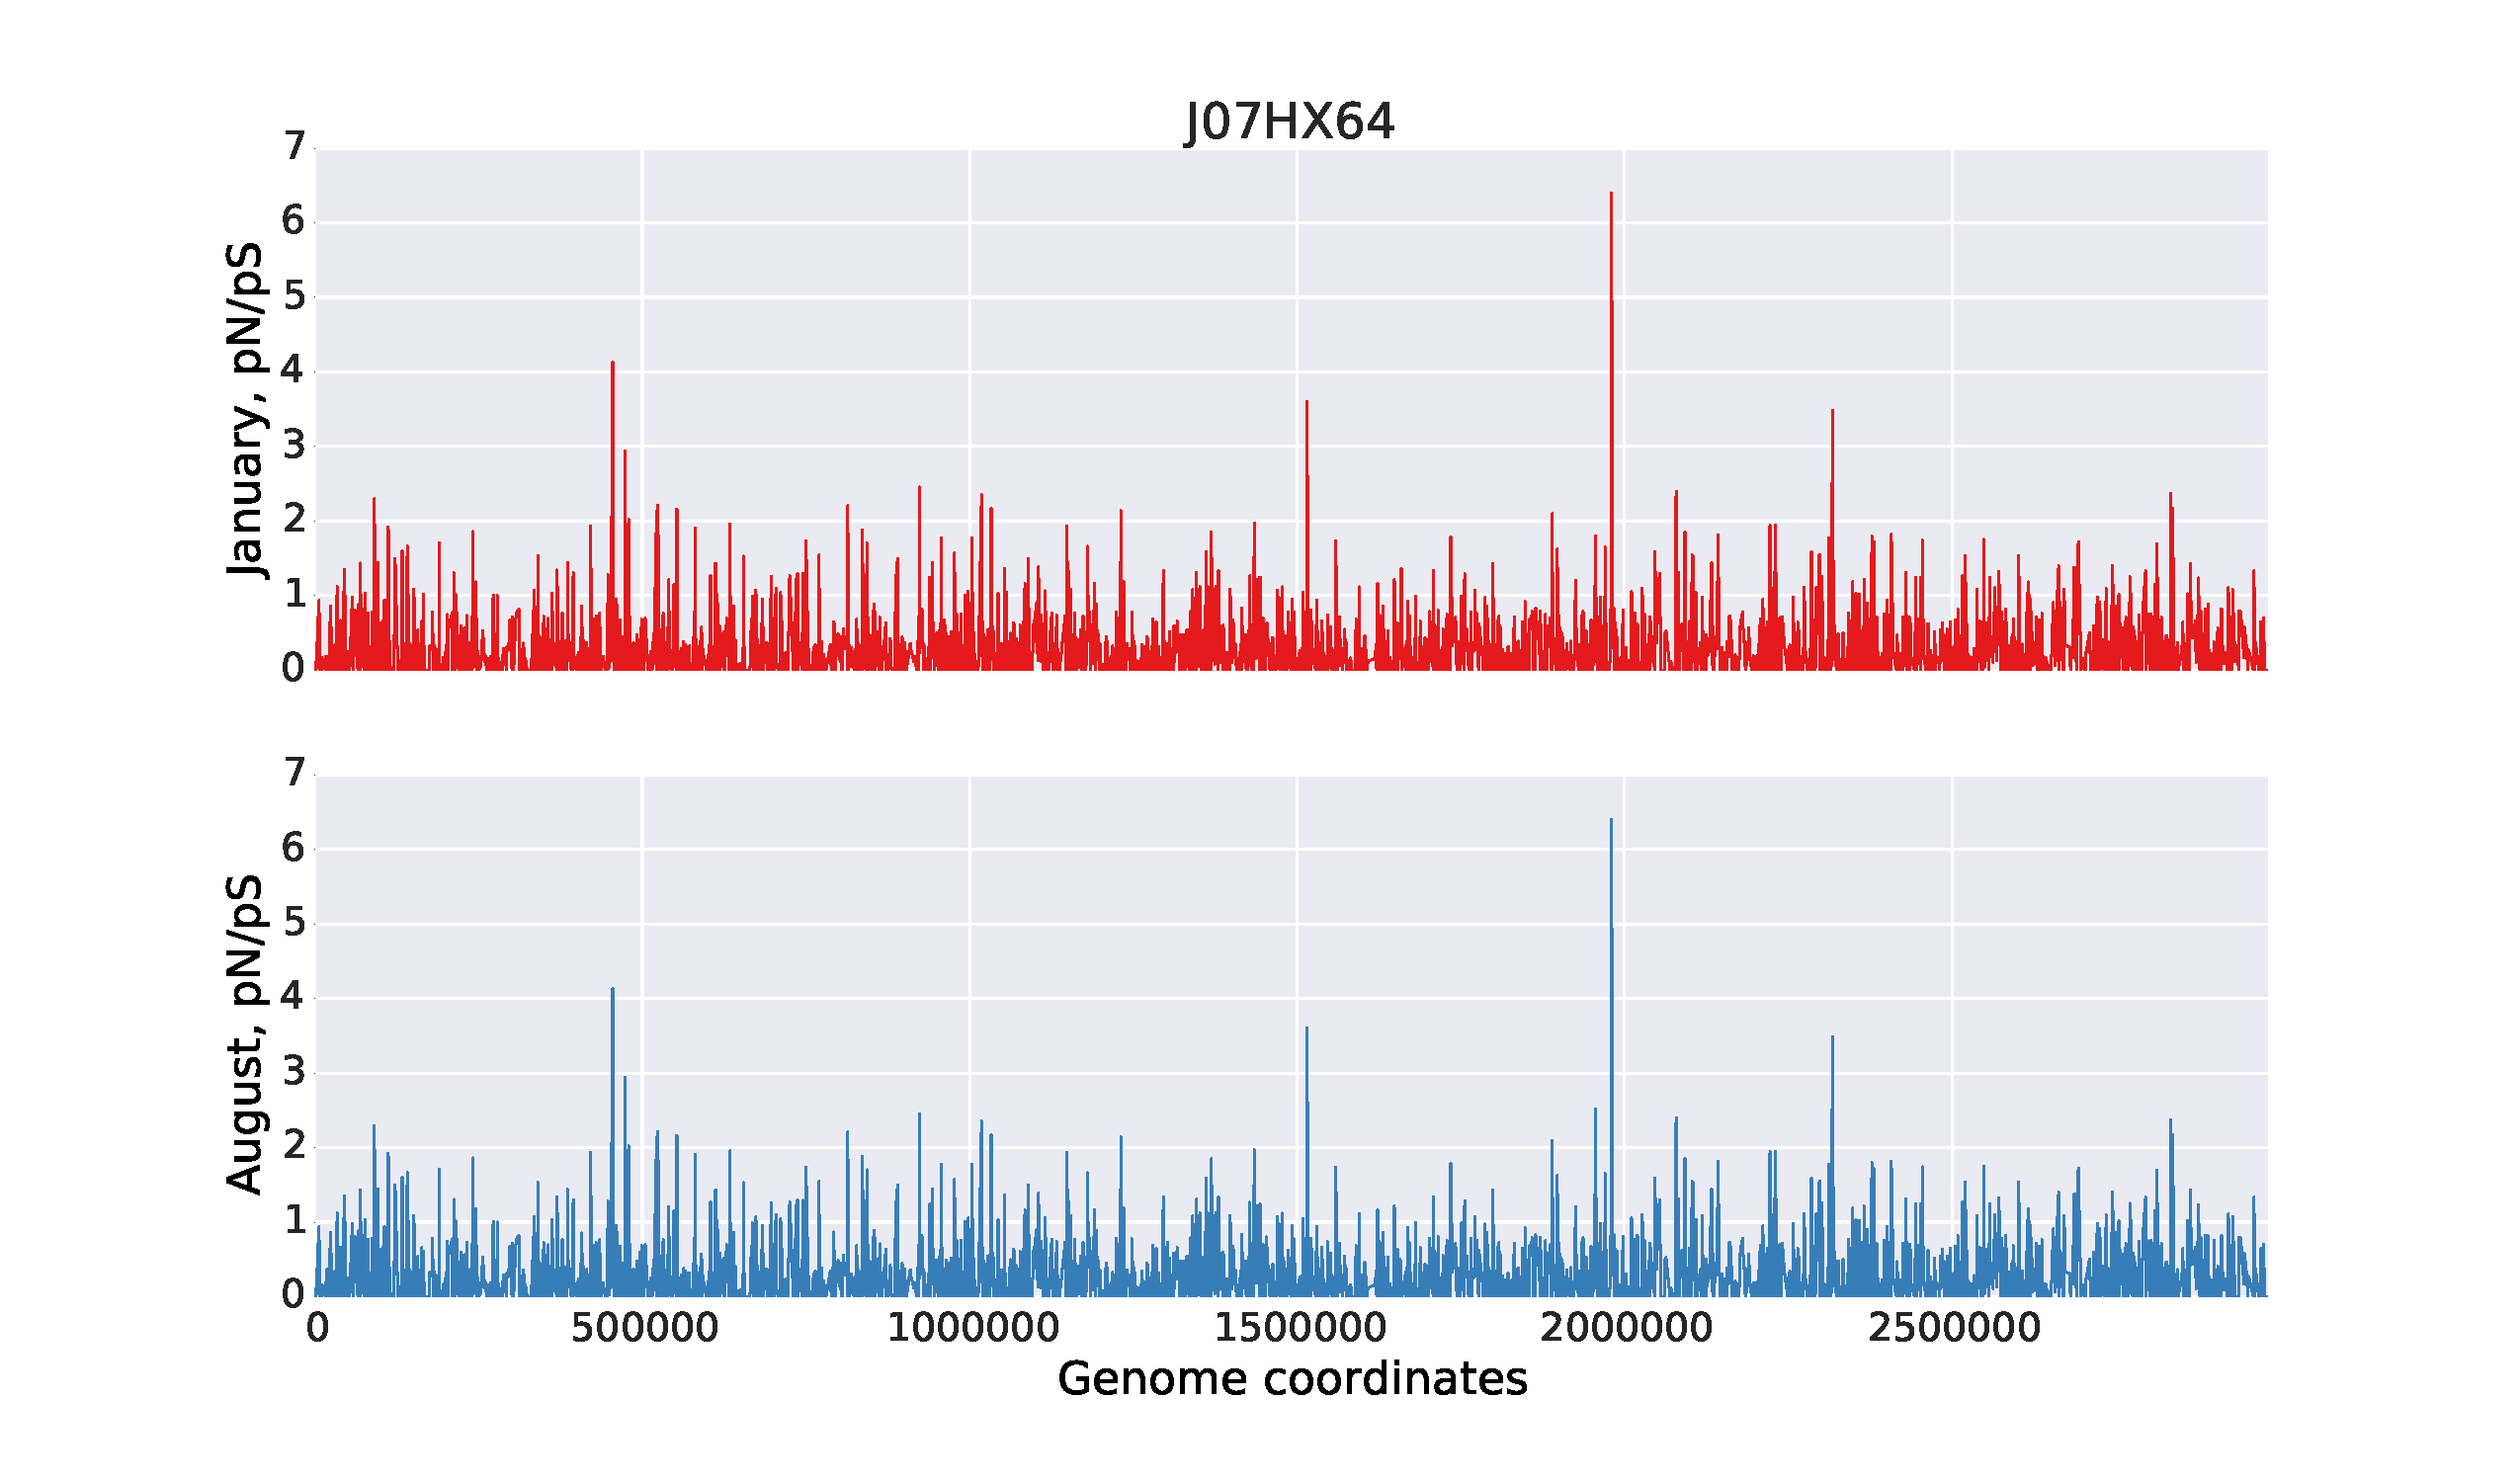
\includegraphics[width=\textwidth,height=\textheight,keepaspectratio]{Chapter5/Figures/pn_ps_plots/J07HX64_pNpS_density.pdf}
  \caption{pN/pS values for each gene in the J07HX64 genome. Top panel shows the values using the reads from the January samples. Bottom panel shows the values using the reads from the August sample}
  \label{J07HX64_pNpS}
\end{figure}

\begin{figure}[p]
  \centering
  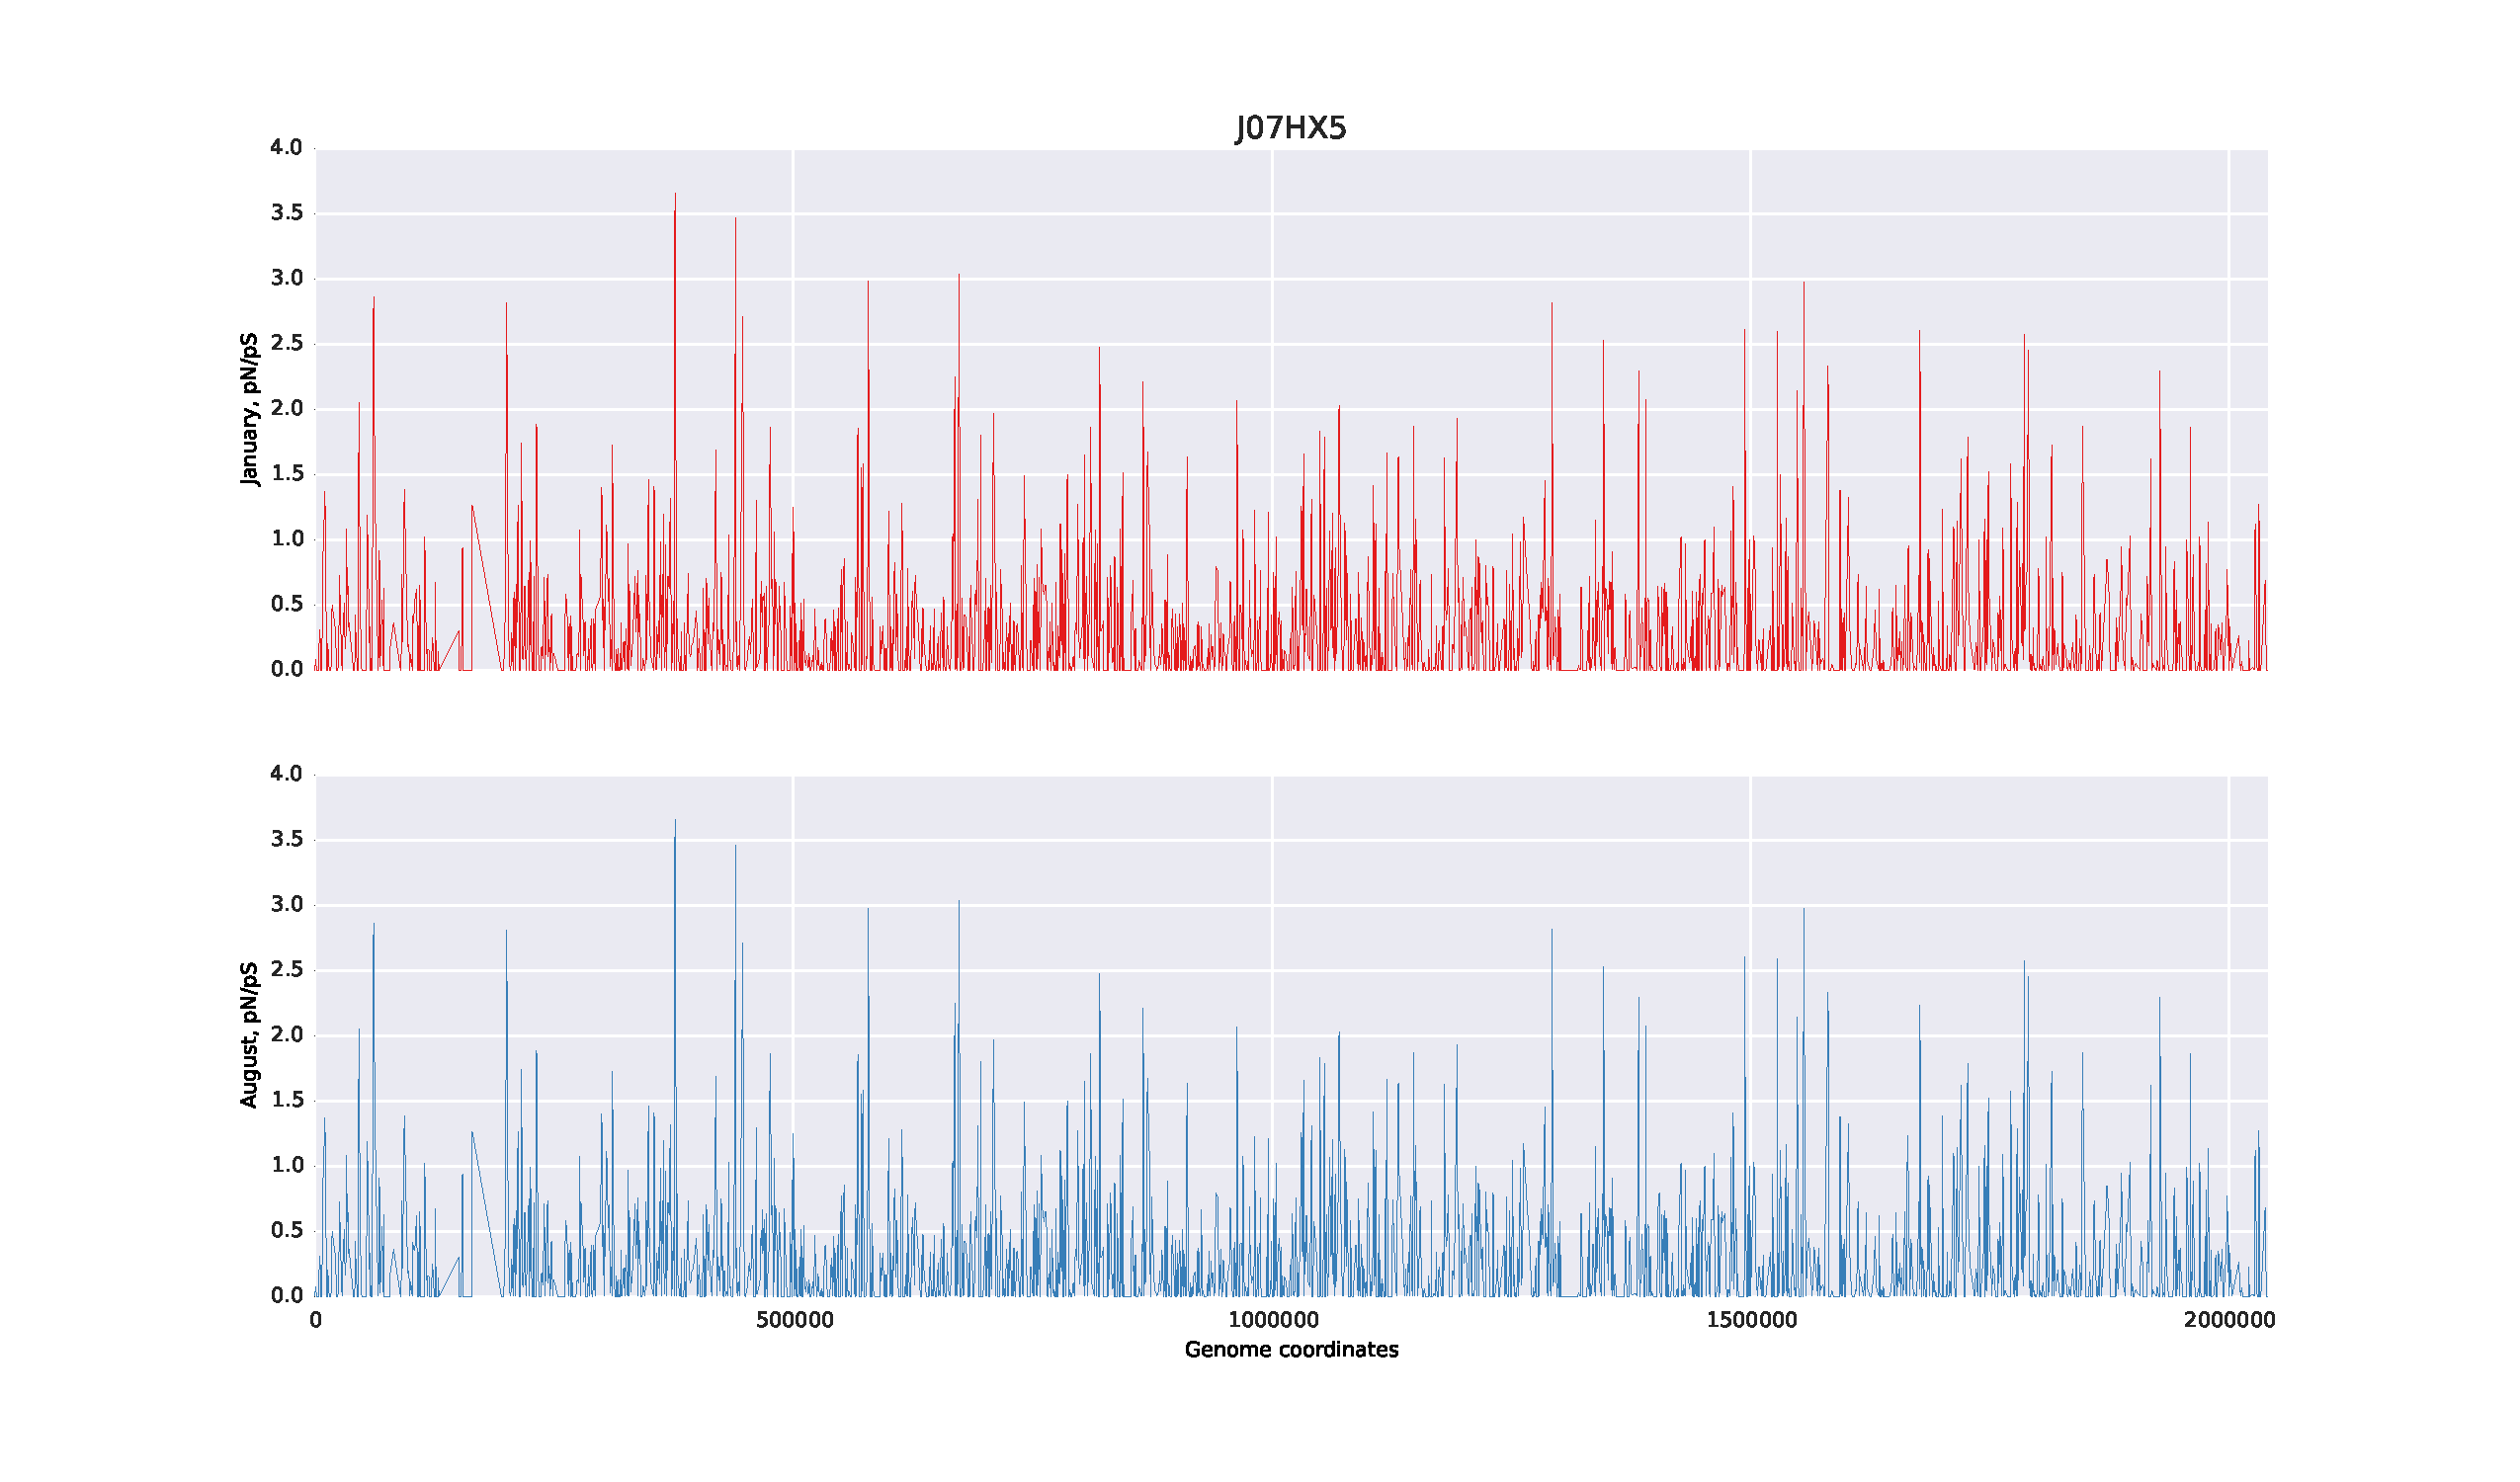
\includegraphics[width=\textwidth,height=\textheight,keepaspectratio]{Chapter5/Figures/pn_ps_plots/J07HX5_pNpS_density.pdf}
  \caption{pN/pS values for each gene in the J07HX5 genome. Top panel shows the values using the reads from the January samples. Bottom panel shows the values using the reads from the August sample}
  \label{J07HX5_pNpS}
\end{figure}

\begin{figure}[p]
  \centering
  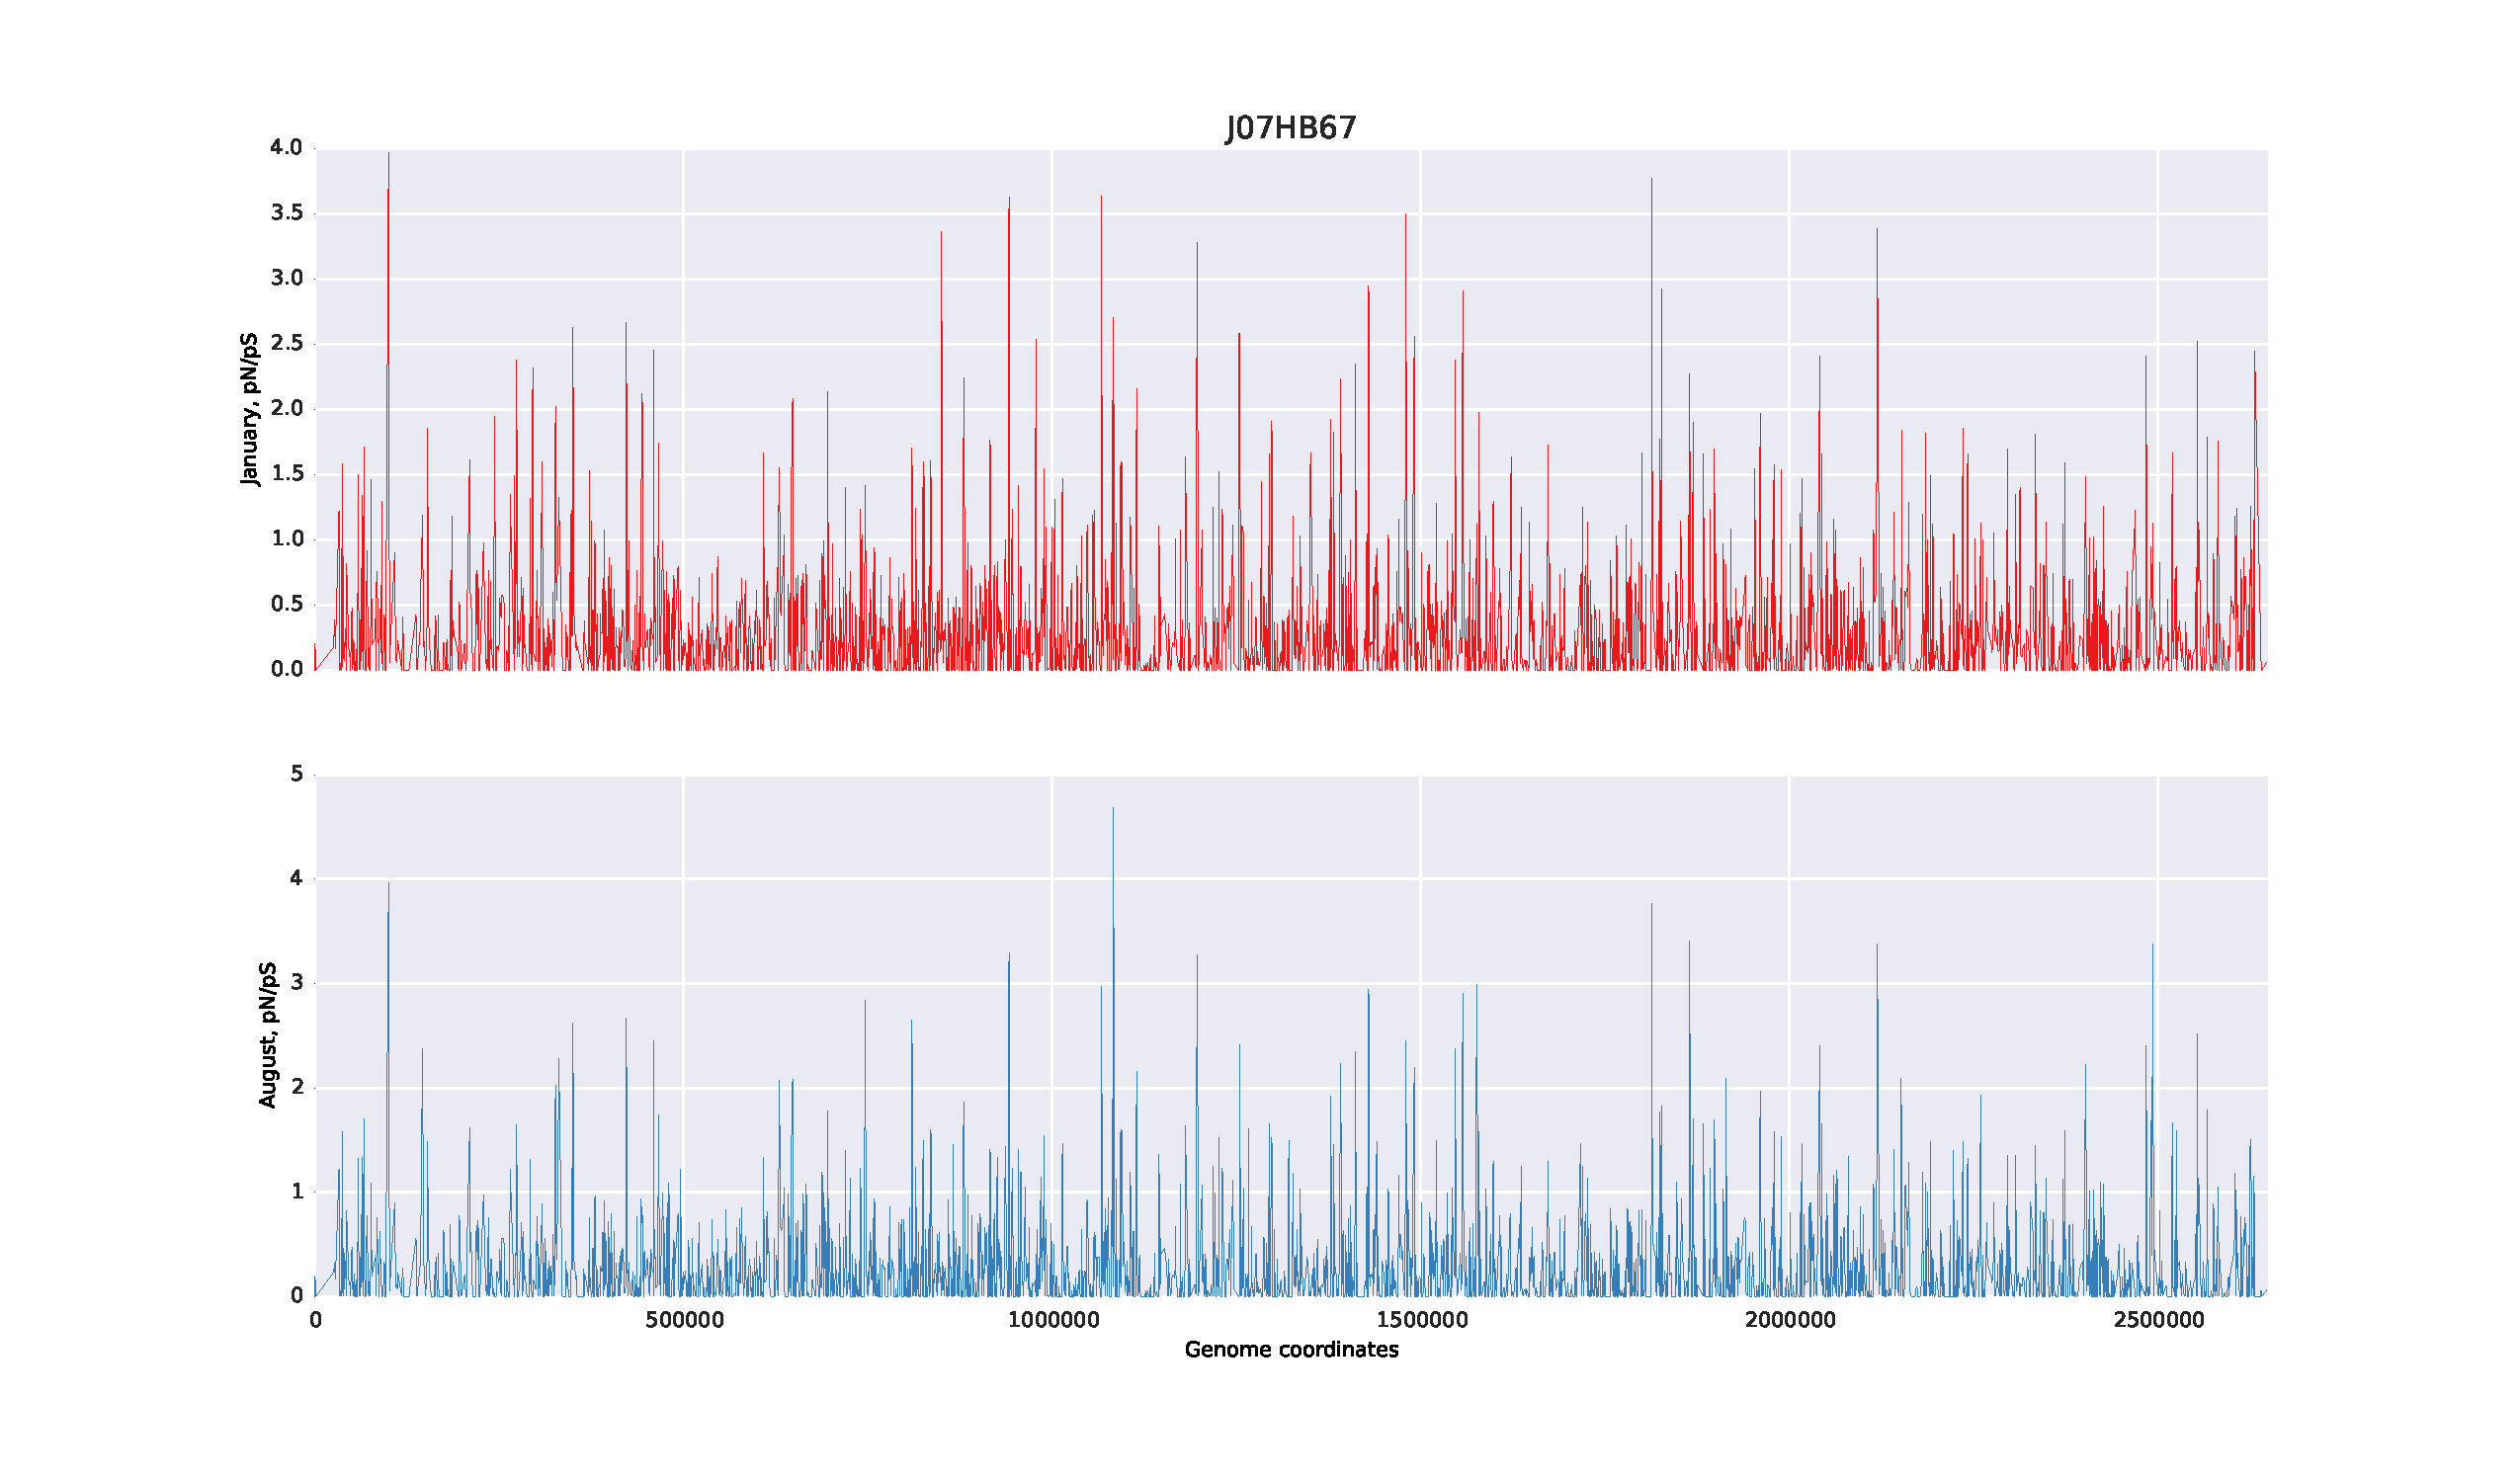
\includegraphics[width=\textwidth,height=\textheight,keepaspectratio]{Chapter5/Figures/pn_ps_plots/J07HB67_pNpS_density.pdf}
  \caption{pN/pS values for each gene in the J07HB67 genome. Top panel shows the values using the reads from the January samples. Bottom panel shows the values using the reads from the August sample}
  \label{J07HB67_pNpS}
\end{figure}

\begin{figure}[p]
  \centering
  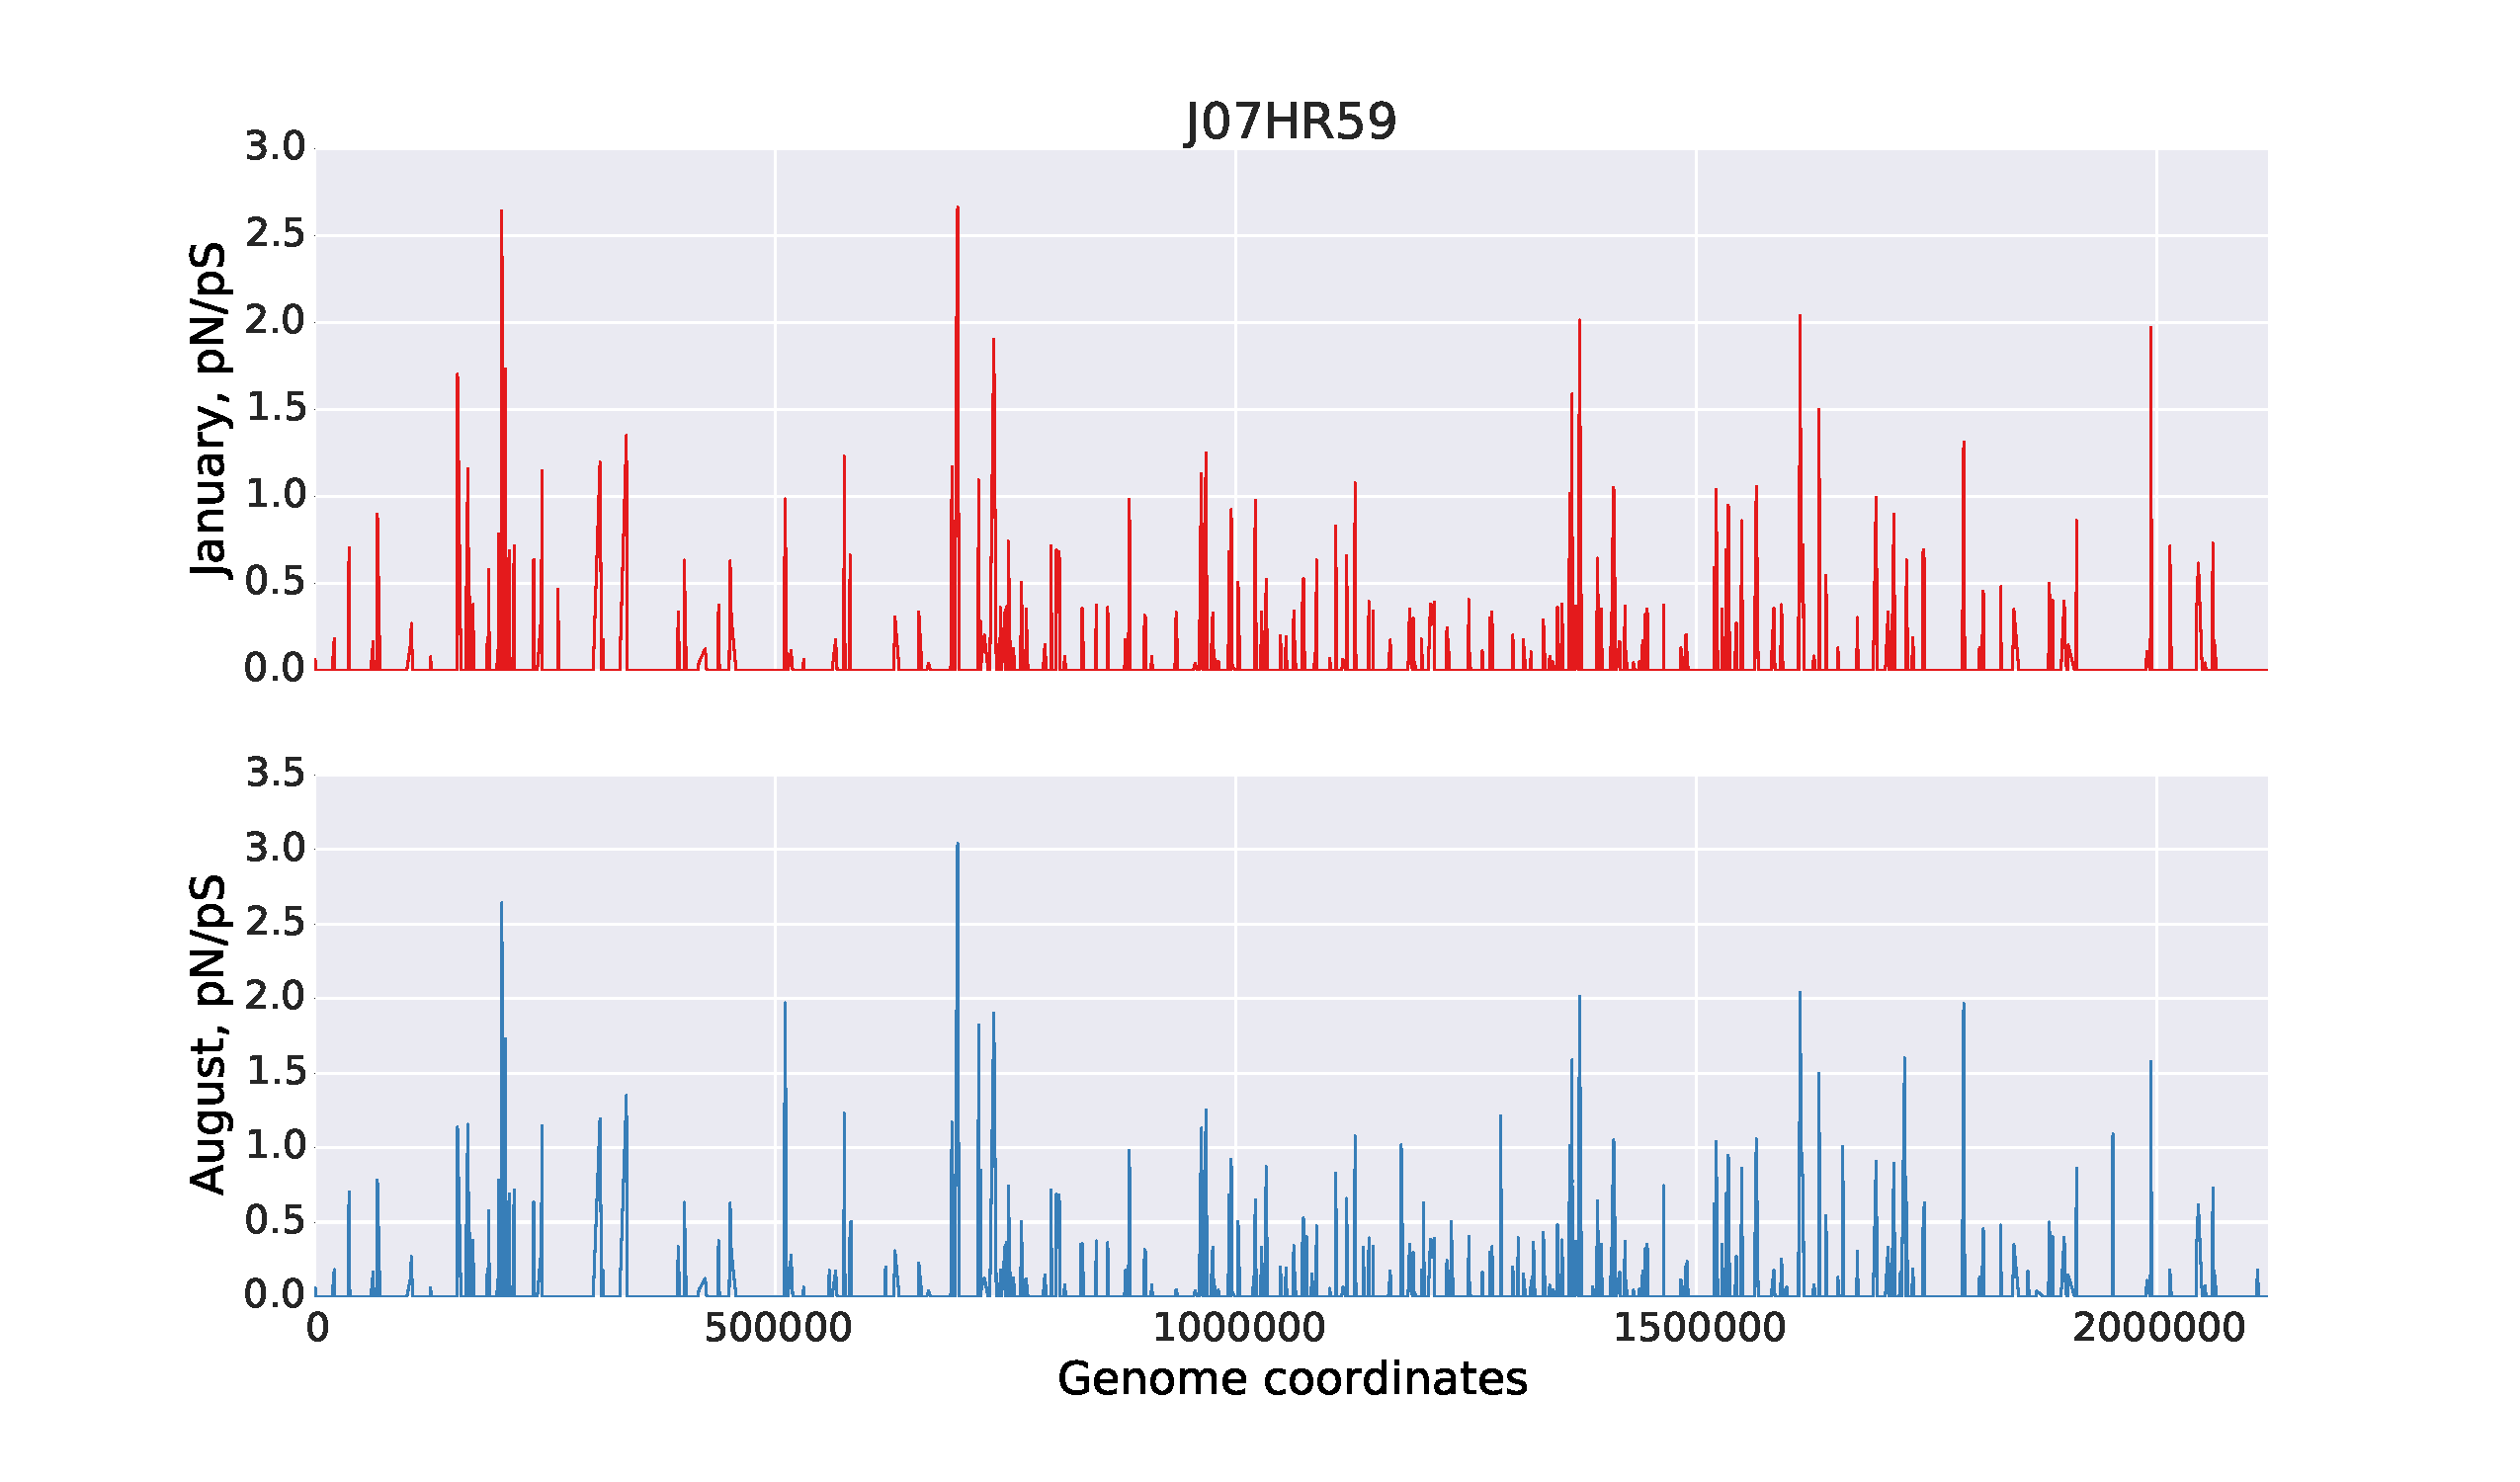
\includegraphics[width=\textwidth,height=\textheight,keepaspectratio]{Chapter5/Figures/pn_ps_plots/J07HR59_pNpS_density.pdf}
  \caption{pN/pS values for each gene in the J07HR59 genome. Top panel shows the values using the reads from the January samples. Bottom panel shows the values using the reads from the August sample}
  \label{J07HR59_pNpS}
\end{figure}

\begin{figure}[p]
  \centering
  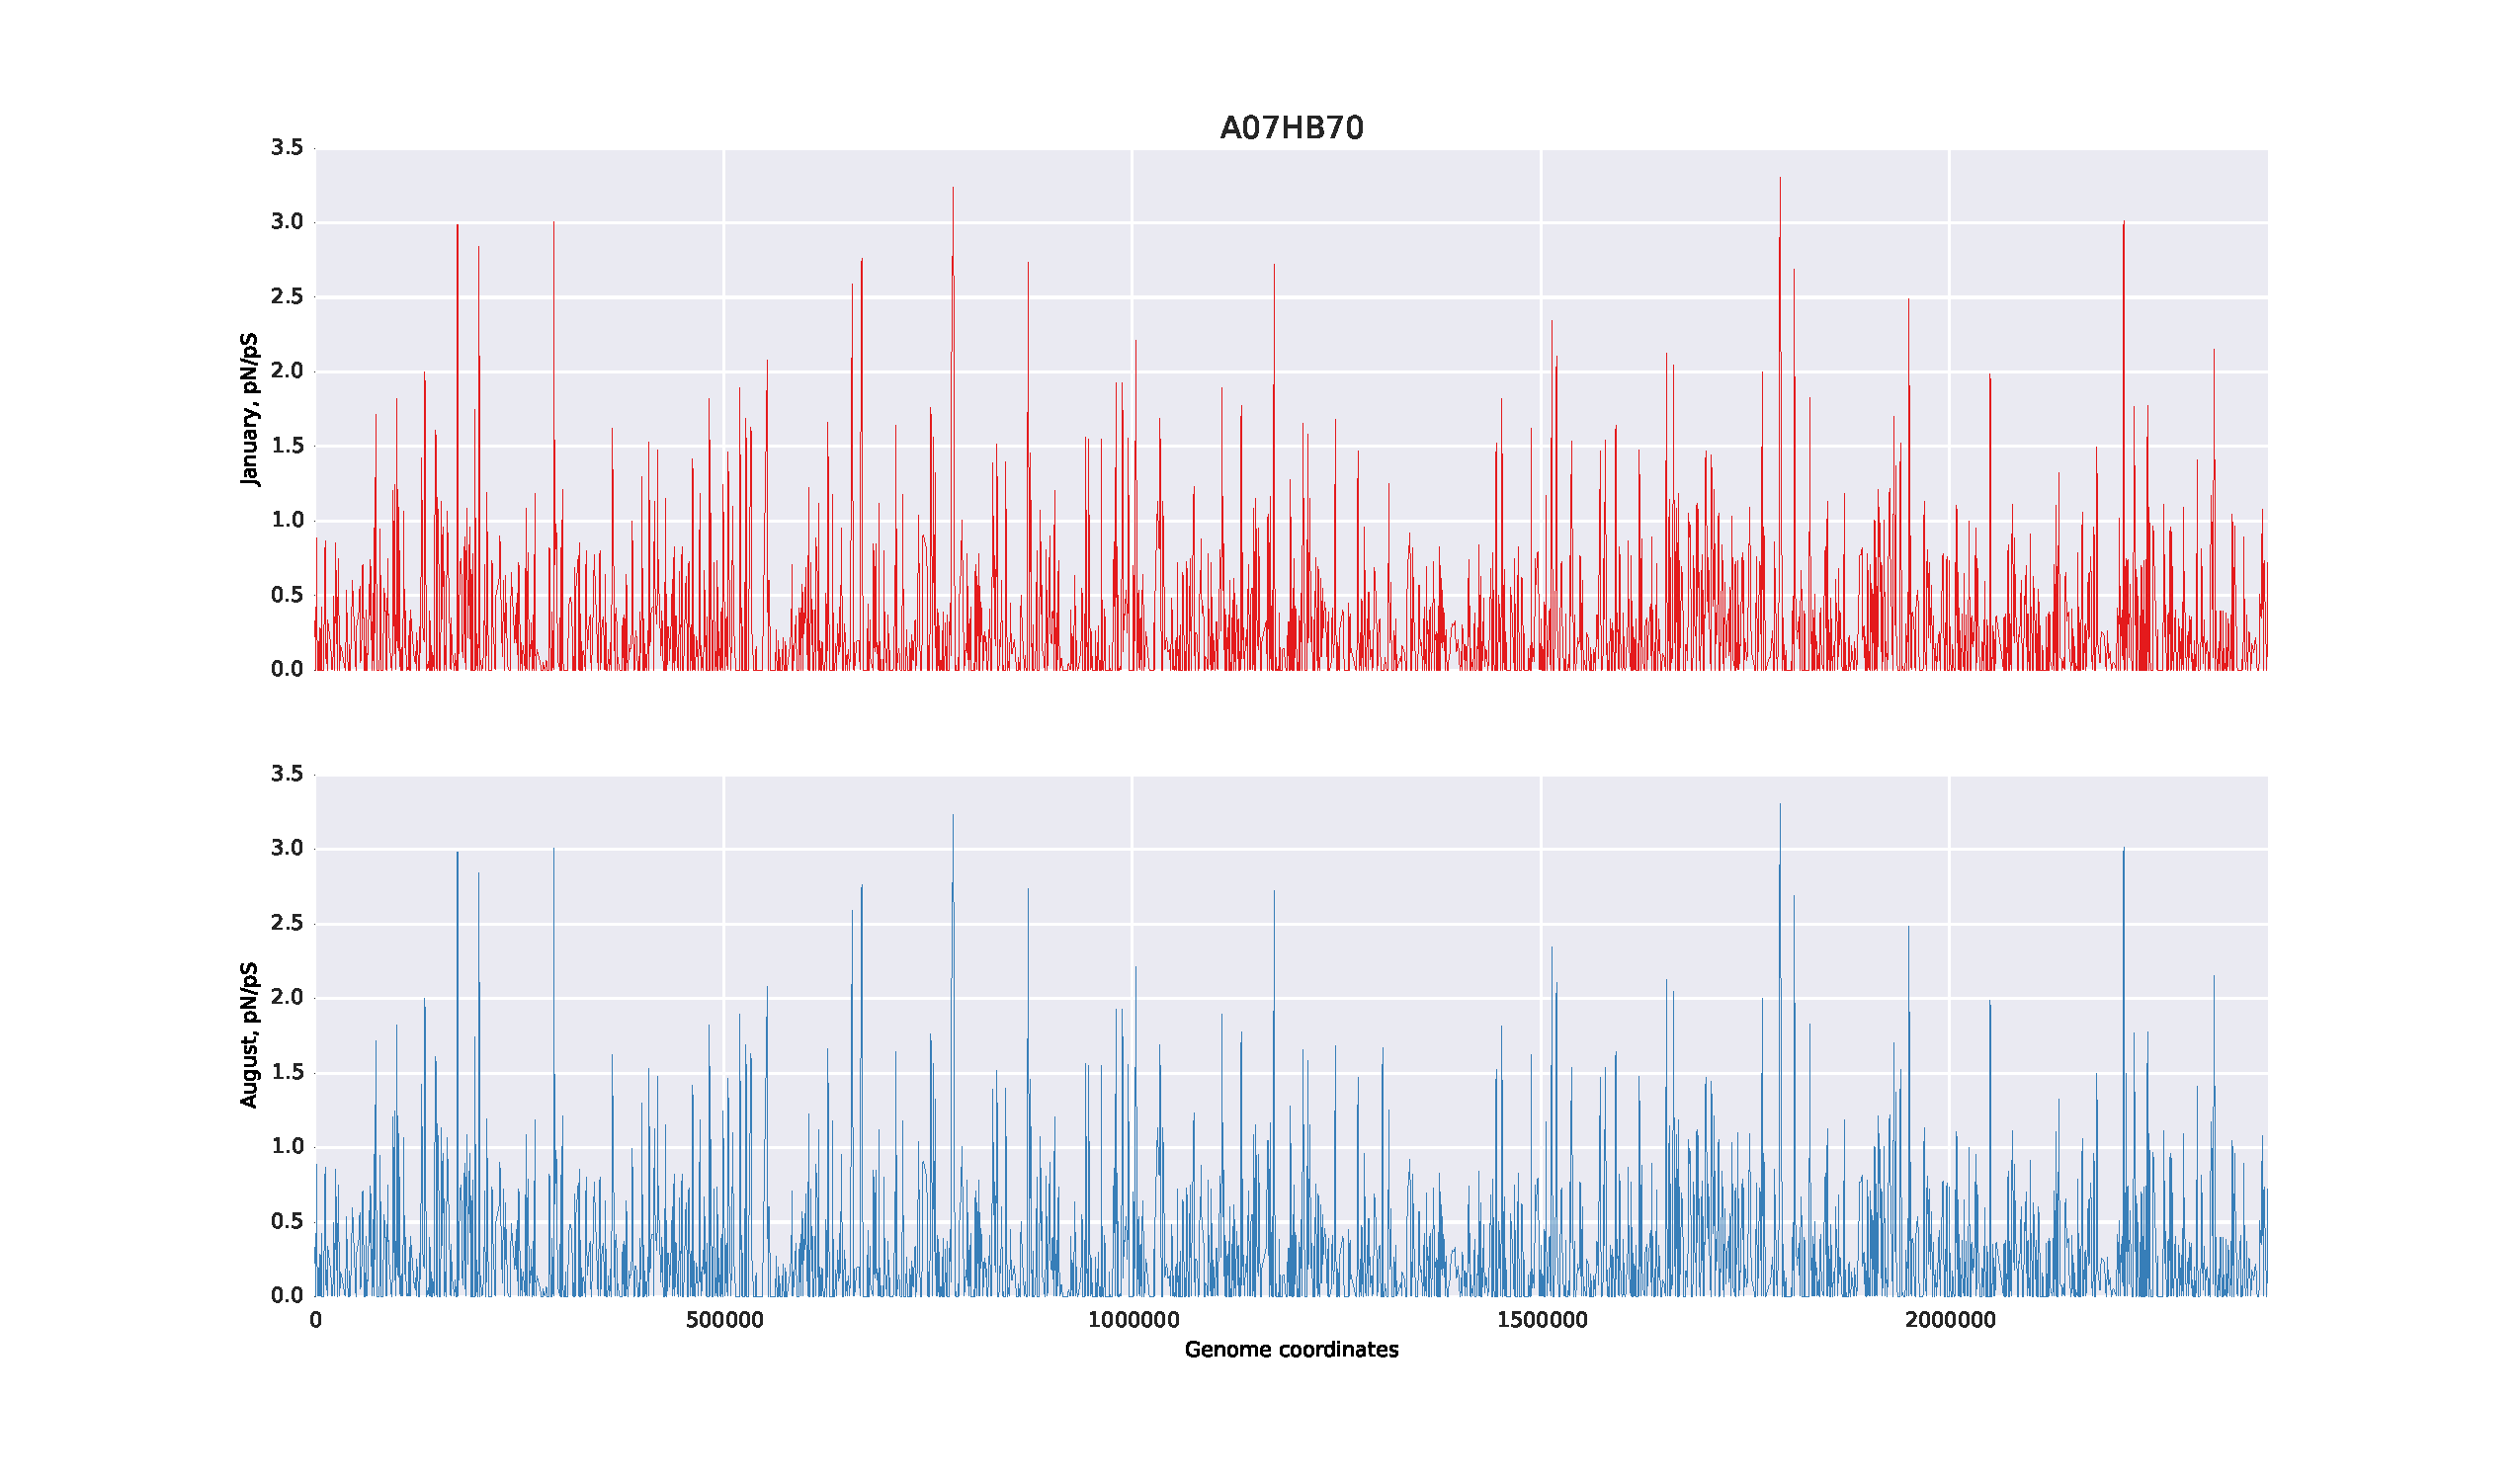
\includegraphics[width=\textwidth,height=\textheight,keepaspectratio]{Chapter5/Figures/pn_ps_plots/A07HB70_pNpS_density.pdf}
  \caption{pN/pS values for each gene in the A07HB70 genome. Top panel shows the values using the reads from the January samples. Bottom panel shows the values using the reads from the August sample}
  \label{A07HB70_pNpS}
\end{figure}

\begin{figure}[p]
  \centering
  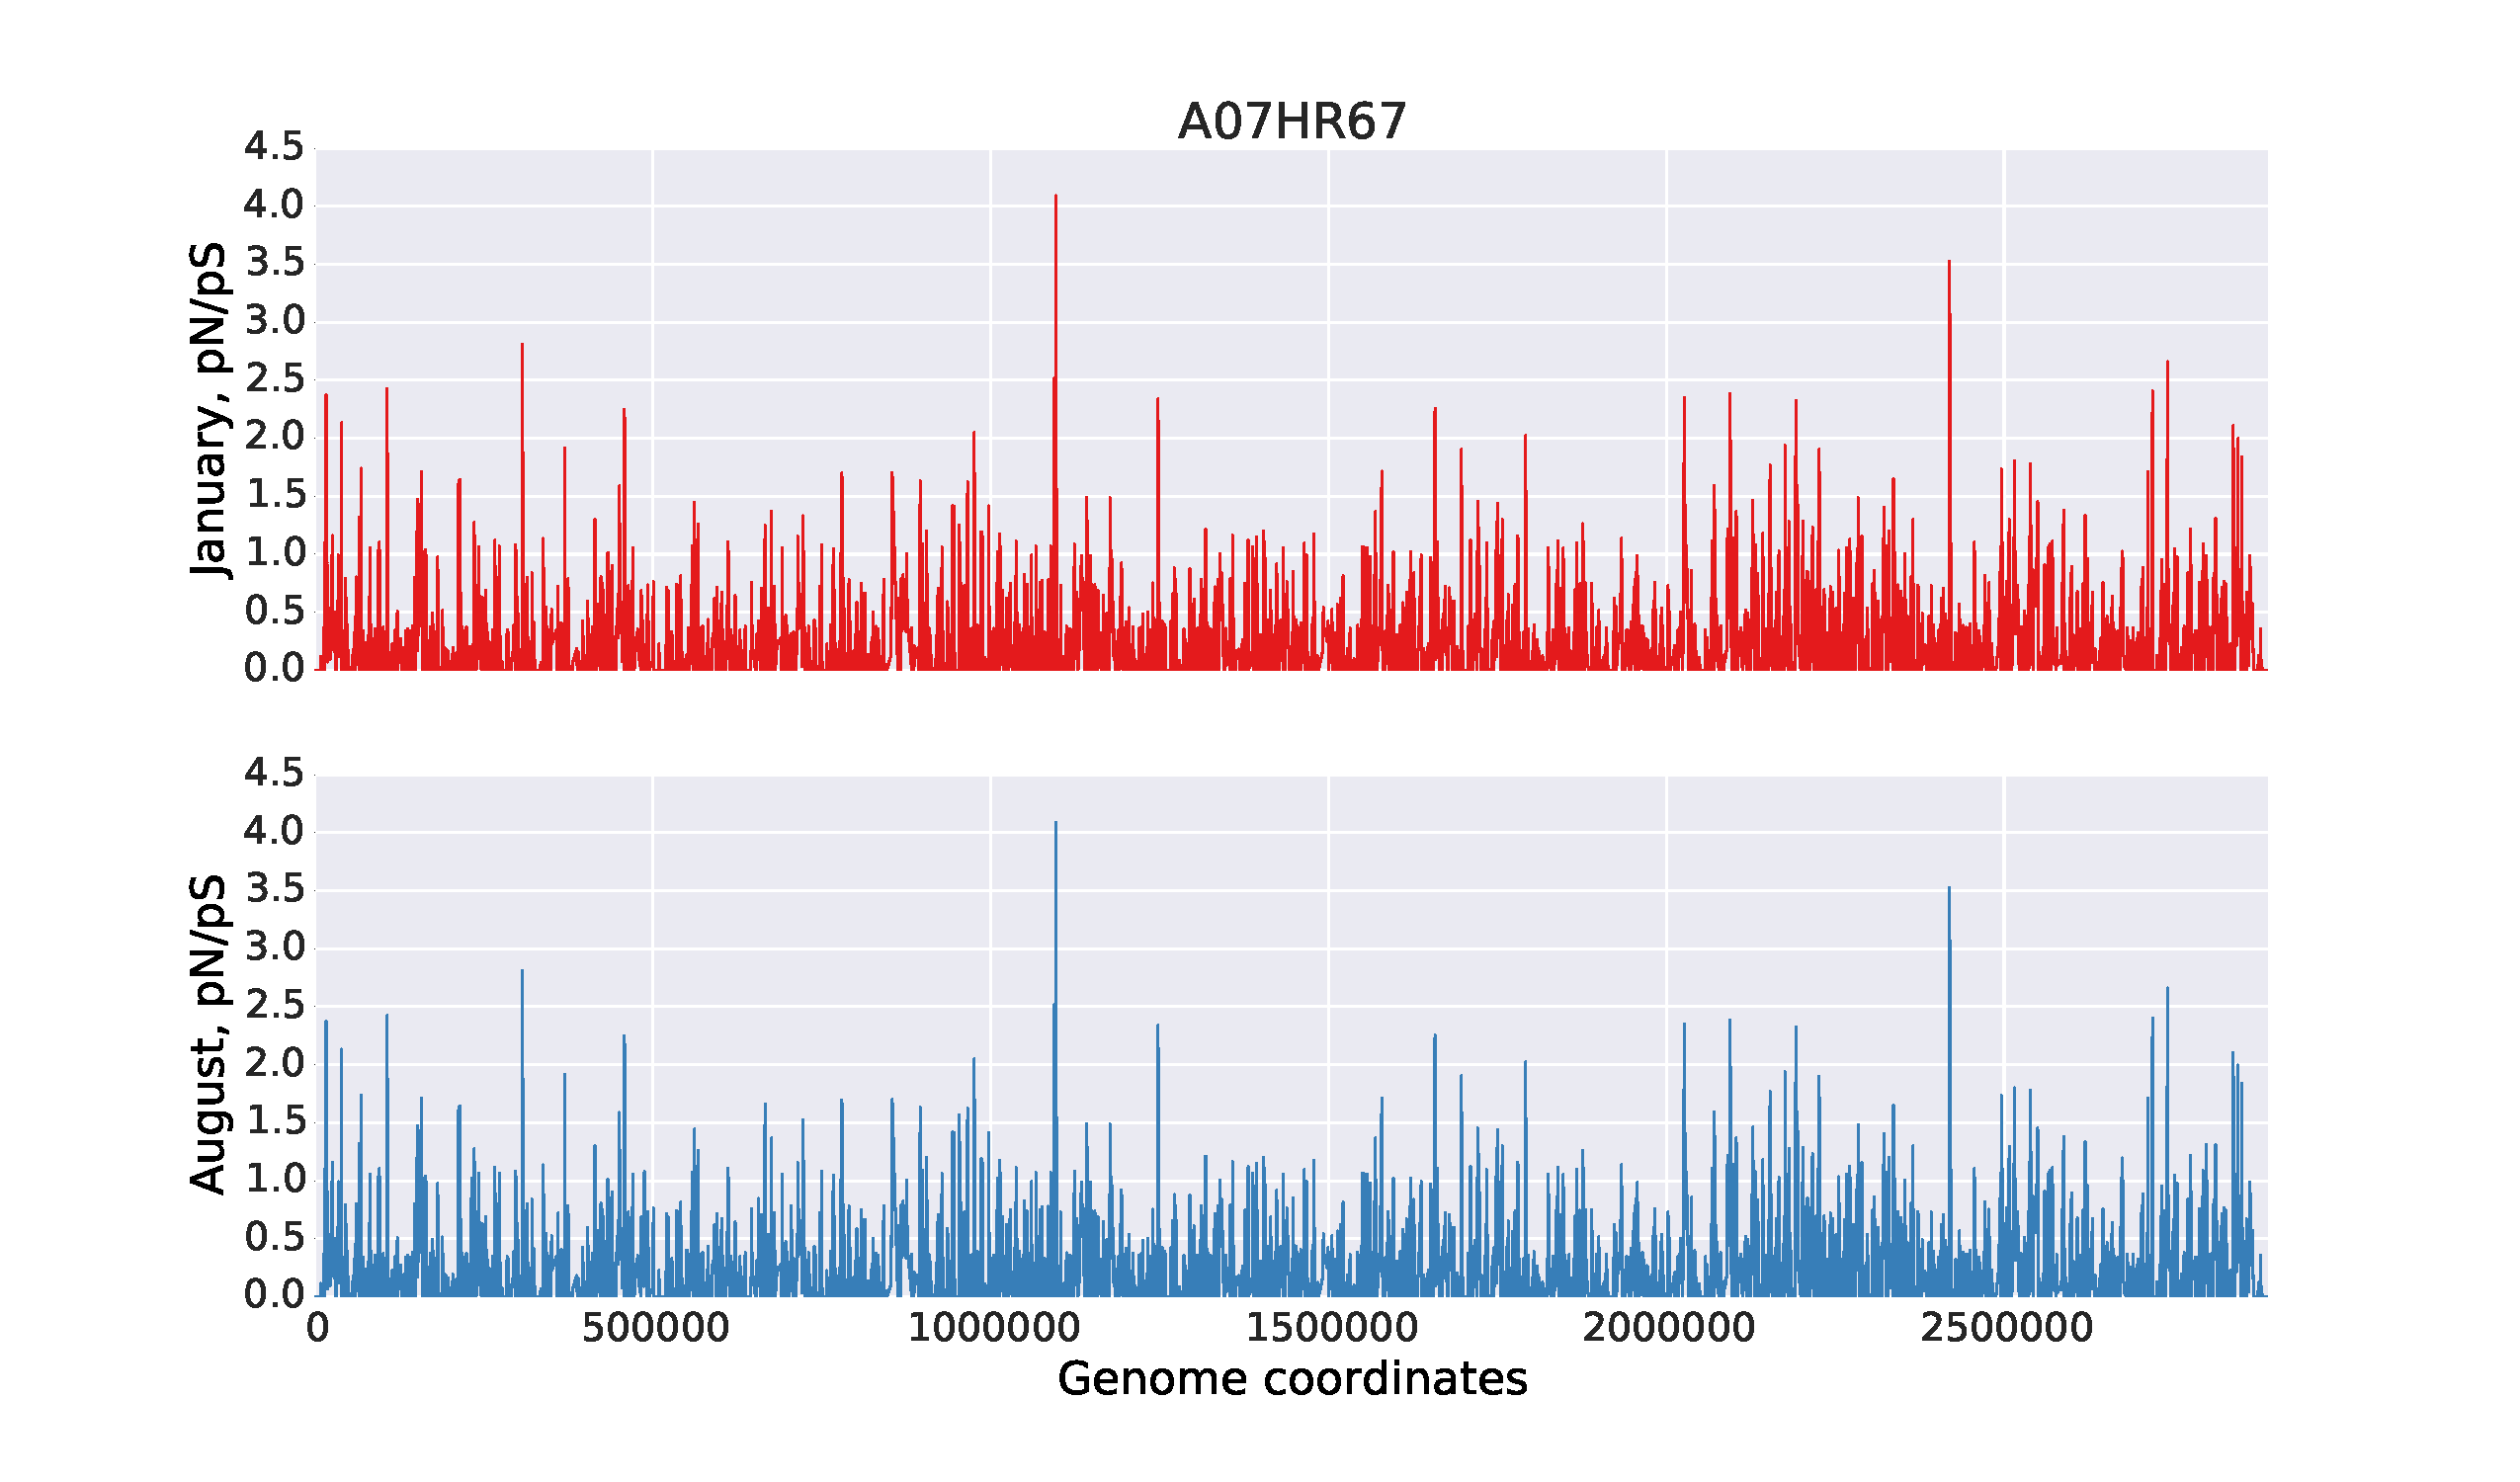
\includegraphics[width=\textwidth,height=\textheight,keepaspectratio]{Chapter5/Figures/pn_ps_plots/A07HR67_pNpS_density.pdf}
  \caption{pN/pS values for each gene in the A07HR67 genome. Top panel shows the values using the reads from the January samples. Bottom panel shows the values using the reads from the August sample}
  \label{A07HR67_pNpS}
\end{figure}

\begin{figure}[p]
  \centering
  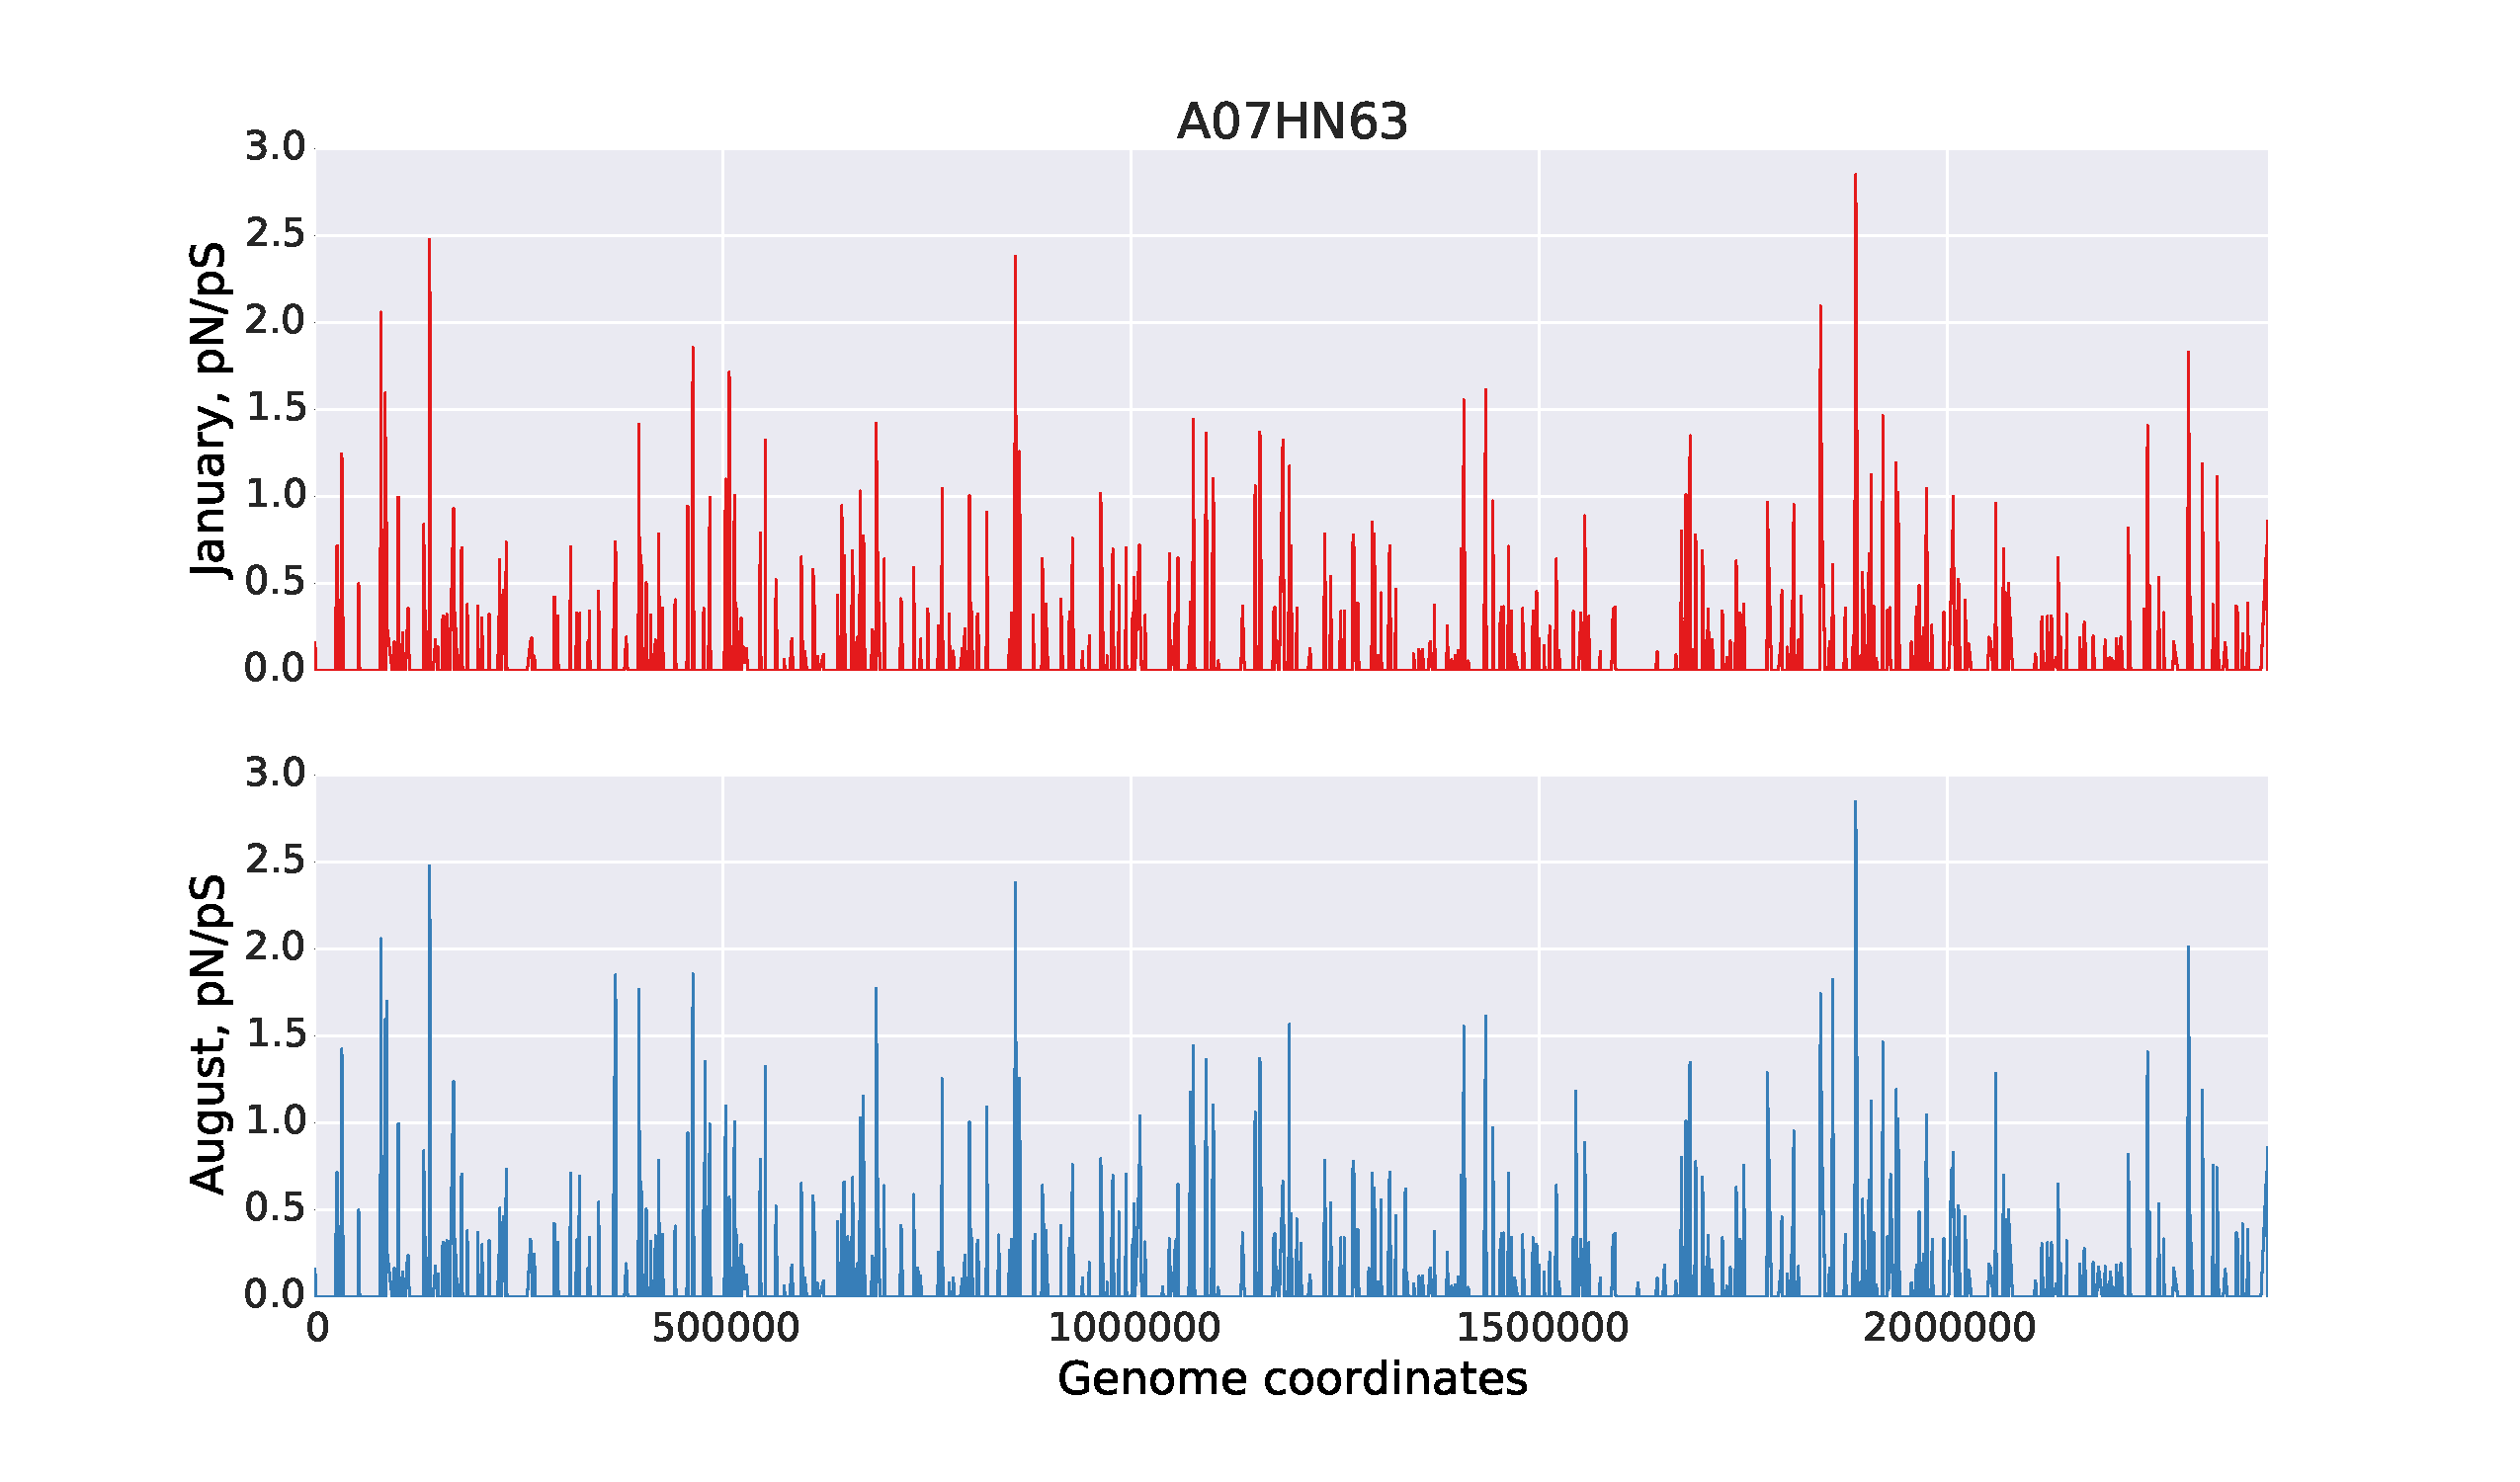
\includegraphics[width=\textwidth,height=\textheight,keepaspectratio]{Chapter5/Figures/pn_ps_plots/A07HN63_pNpS_density.pdf}
  \caption{pN/pS values for each gene in the A07HN63 genome. Top panel shows the values using the reads from the January samples. Bottom panel shows the values using the reads from the August sample}
  \label{A07HN63_pNpS}
\end{figure}

\begin{figure}[p]
  \centering
  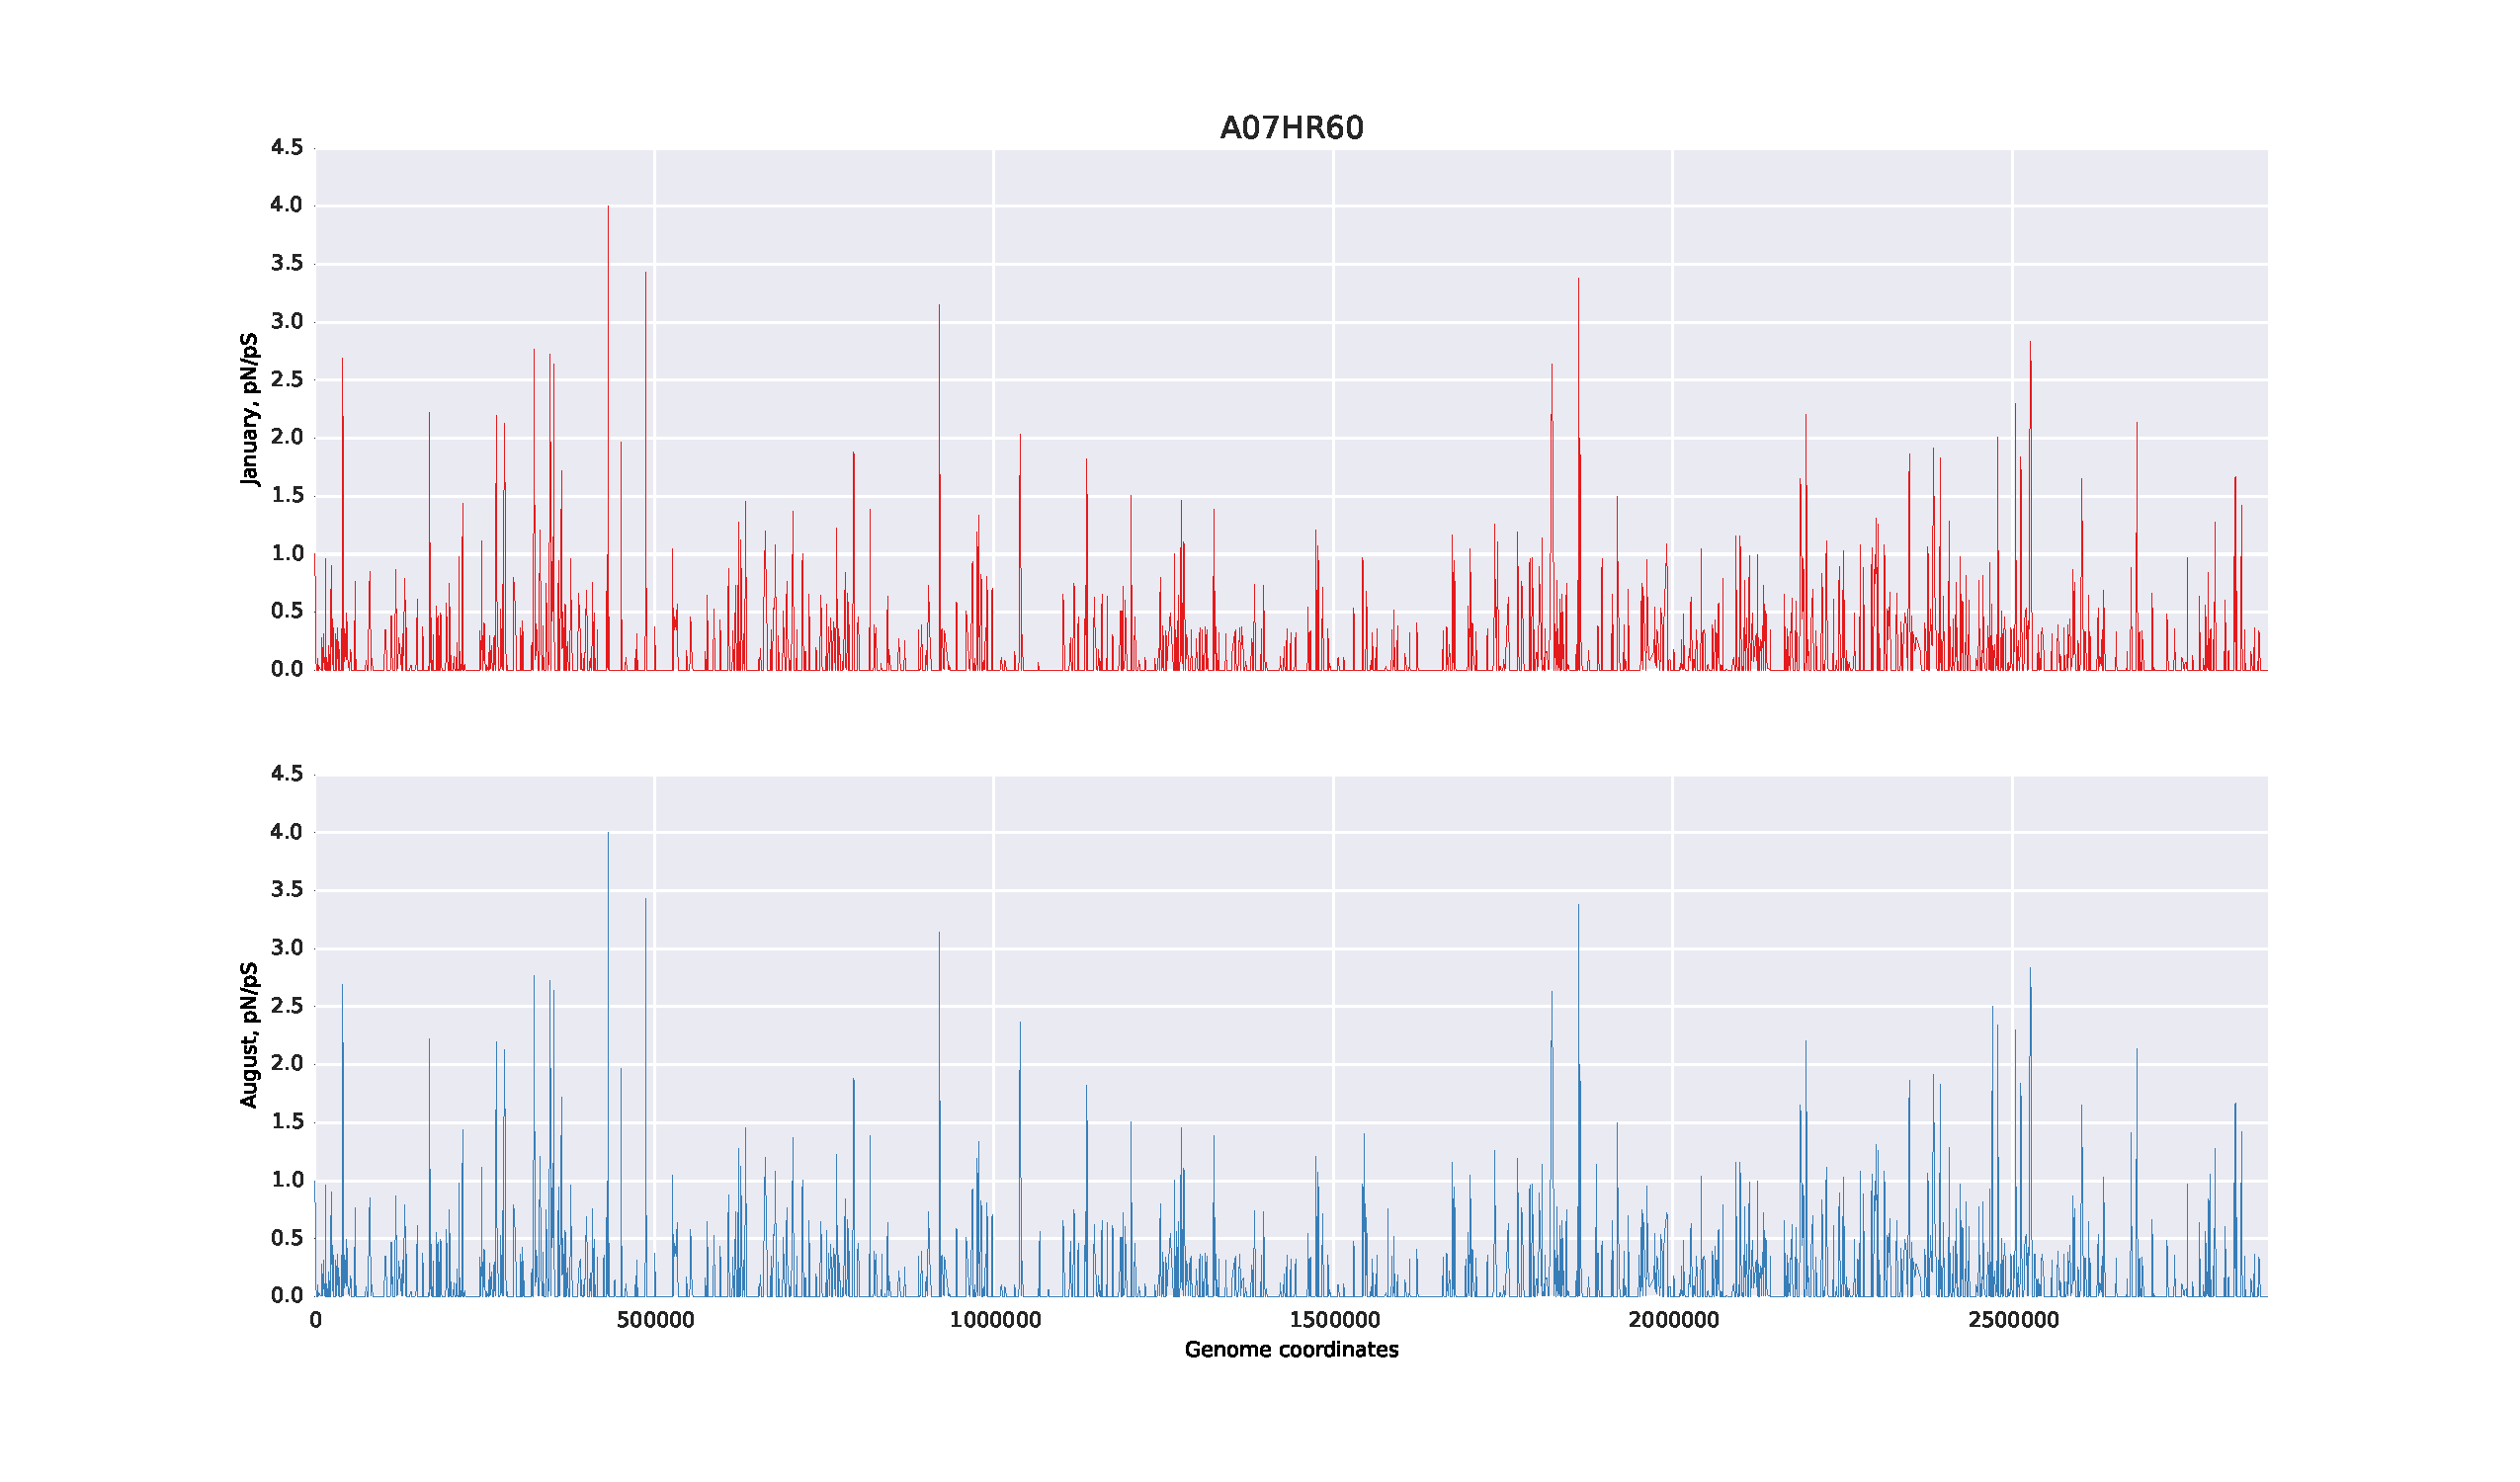
\includegraphics[width=\textwidth,height=\textheight,keepaspectratio]{Chapter5/Figures/pn_ps_plots/A07HR60_pNpS_density.pdf}
  \caption{pN/pS values for each gene in the A07HR60 genome. Top panel shows the values using the reads from the January samples. Bottom panel shows the values using the reads from the August sample}
  \label{A07HR60_pNpS}
\end{figure}

\begin{figure}[p]
  \centering
  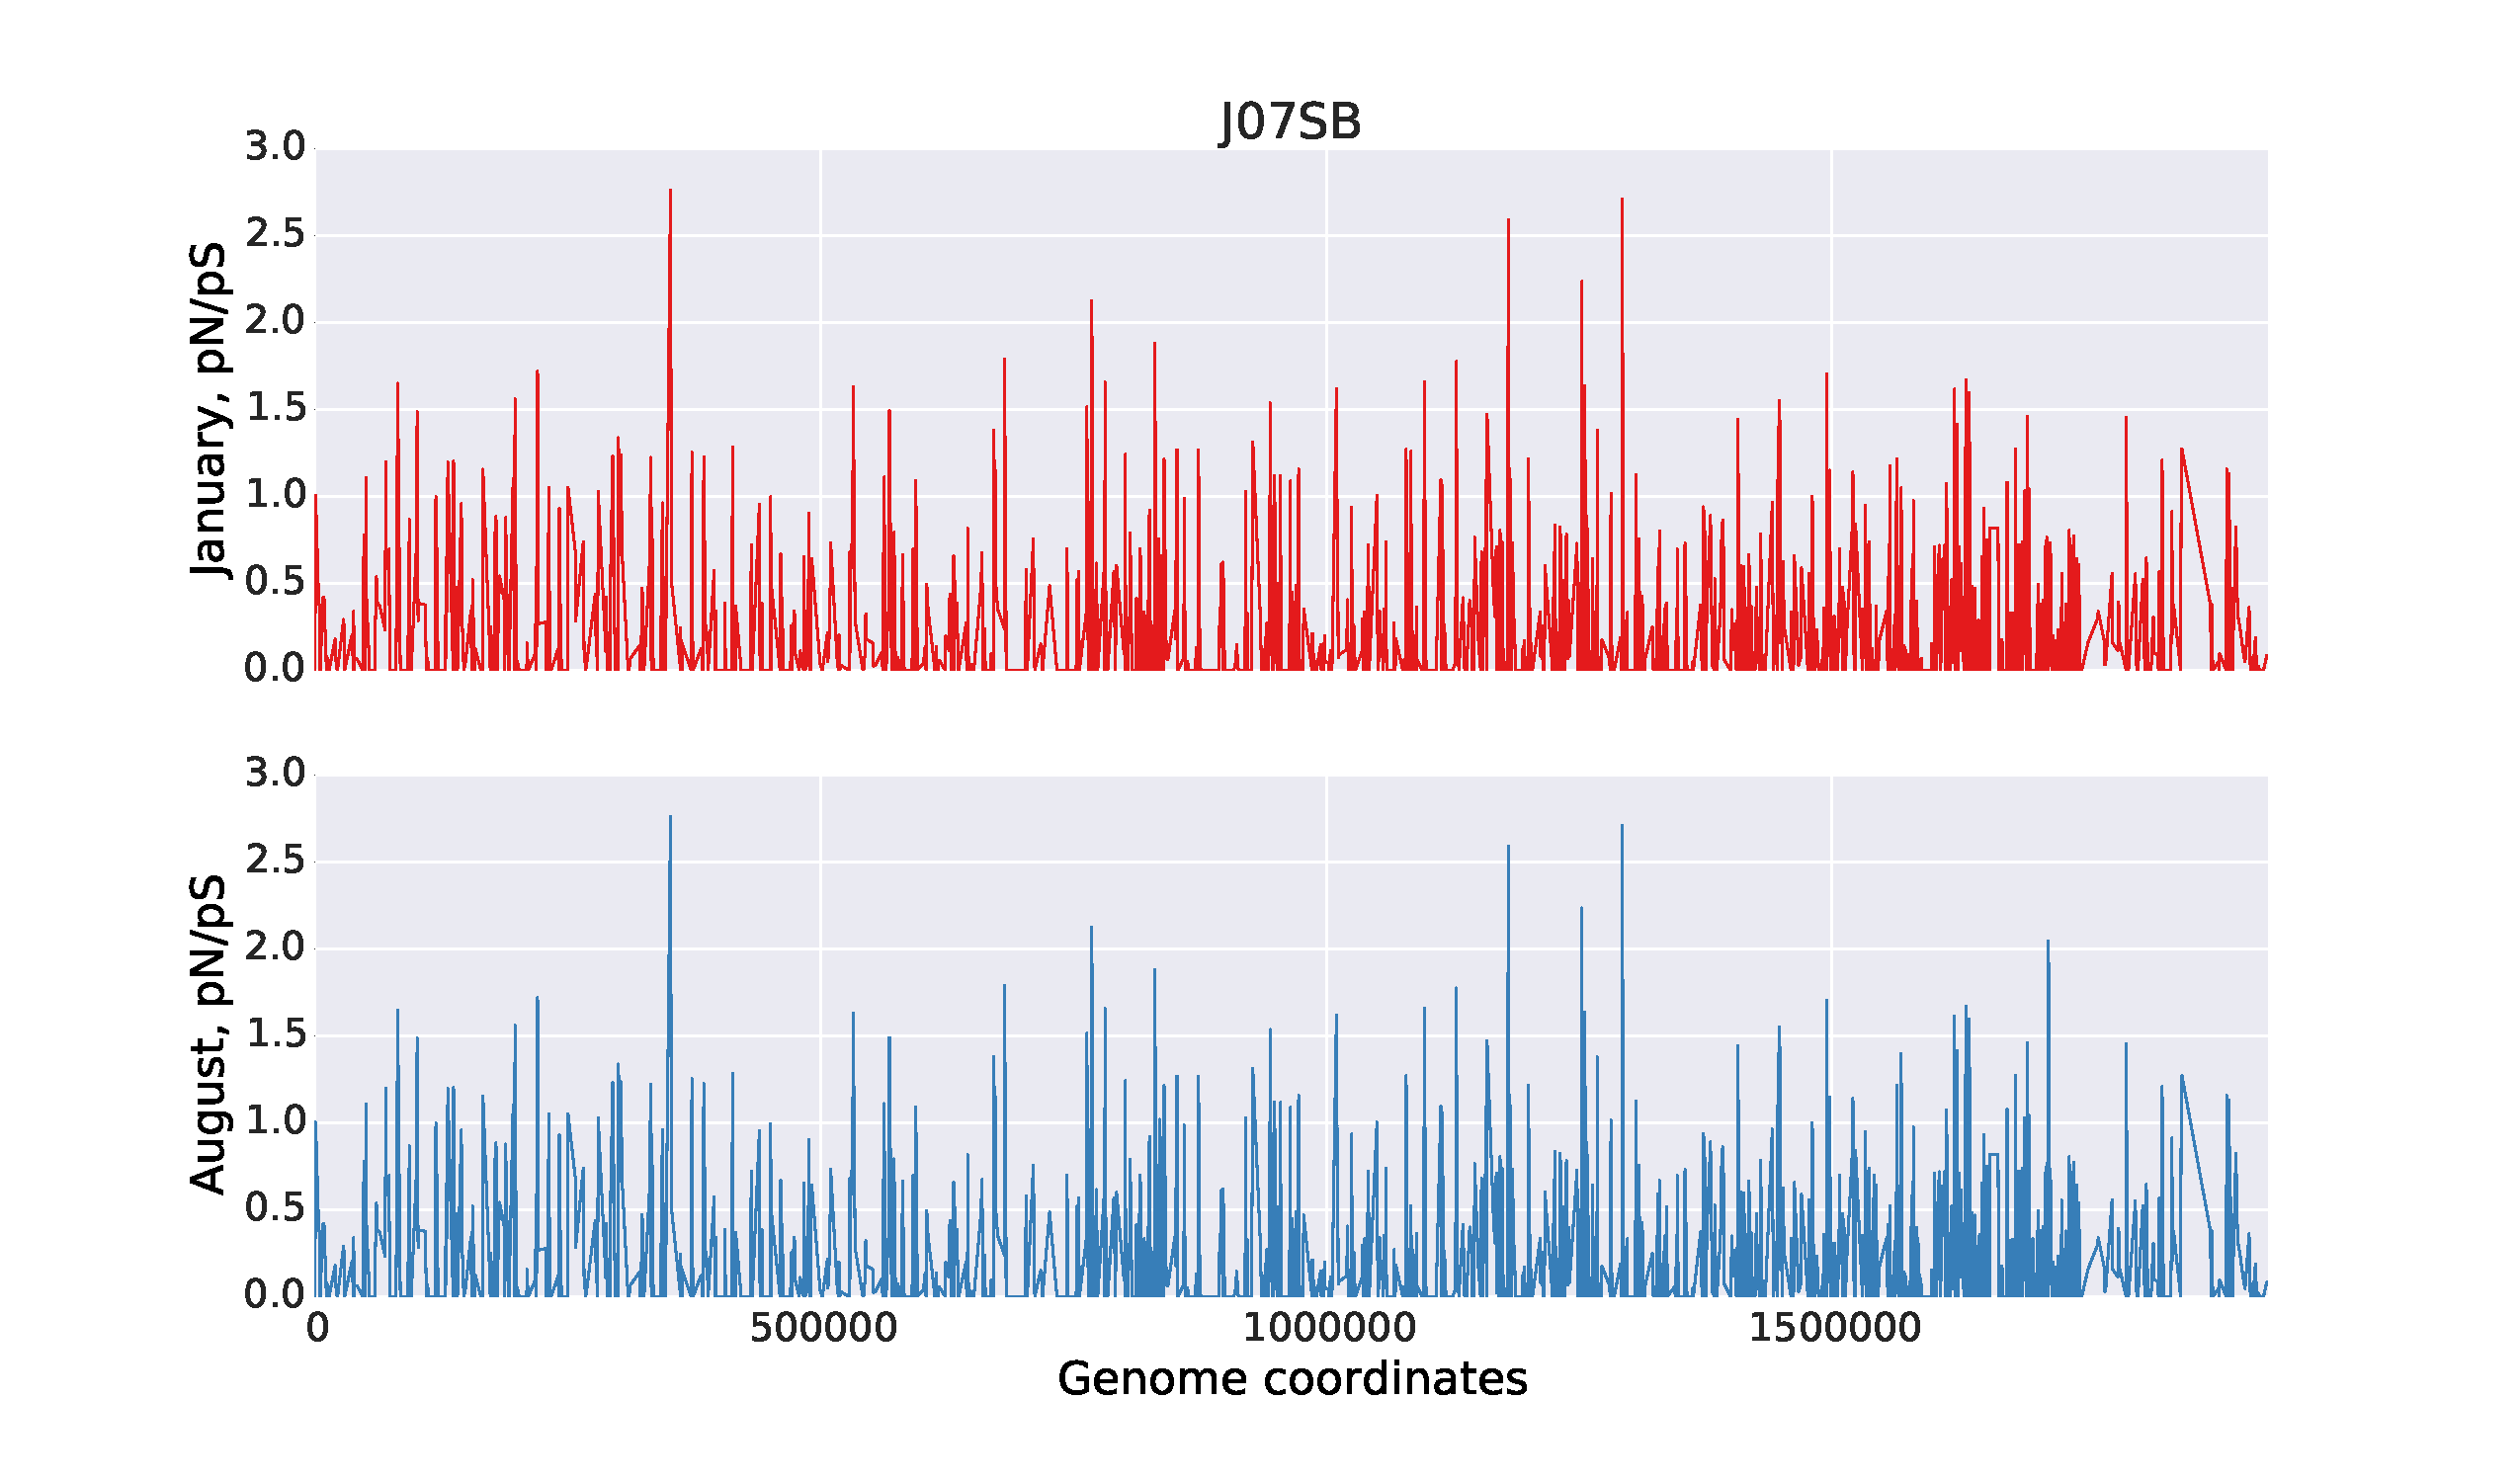
\includegraphics[width=\textwidth,height=\textheight,keepaspectratio]{Chapter5/Figures/pn_ps_plots/J07SB_pNpS_density.pdf}
  \caption{pN/pS values for each gene in the J07SB genome. Top panel shows the values using the reads from the January samples. Bottom panel shows the values using the reads from the August sample}
  \label{J07SB_pNpS}
\end{figure}

\begin{figure}[p]
  \centering
  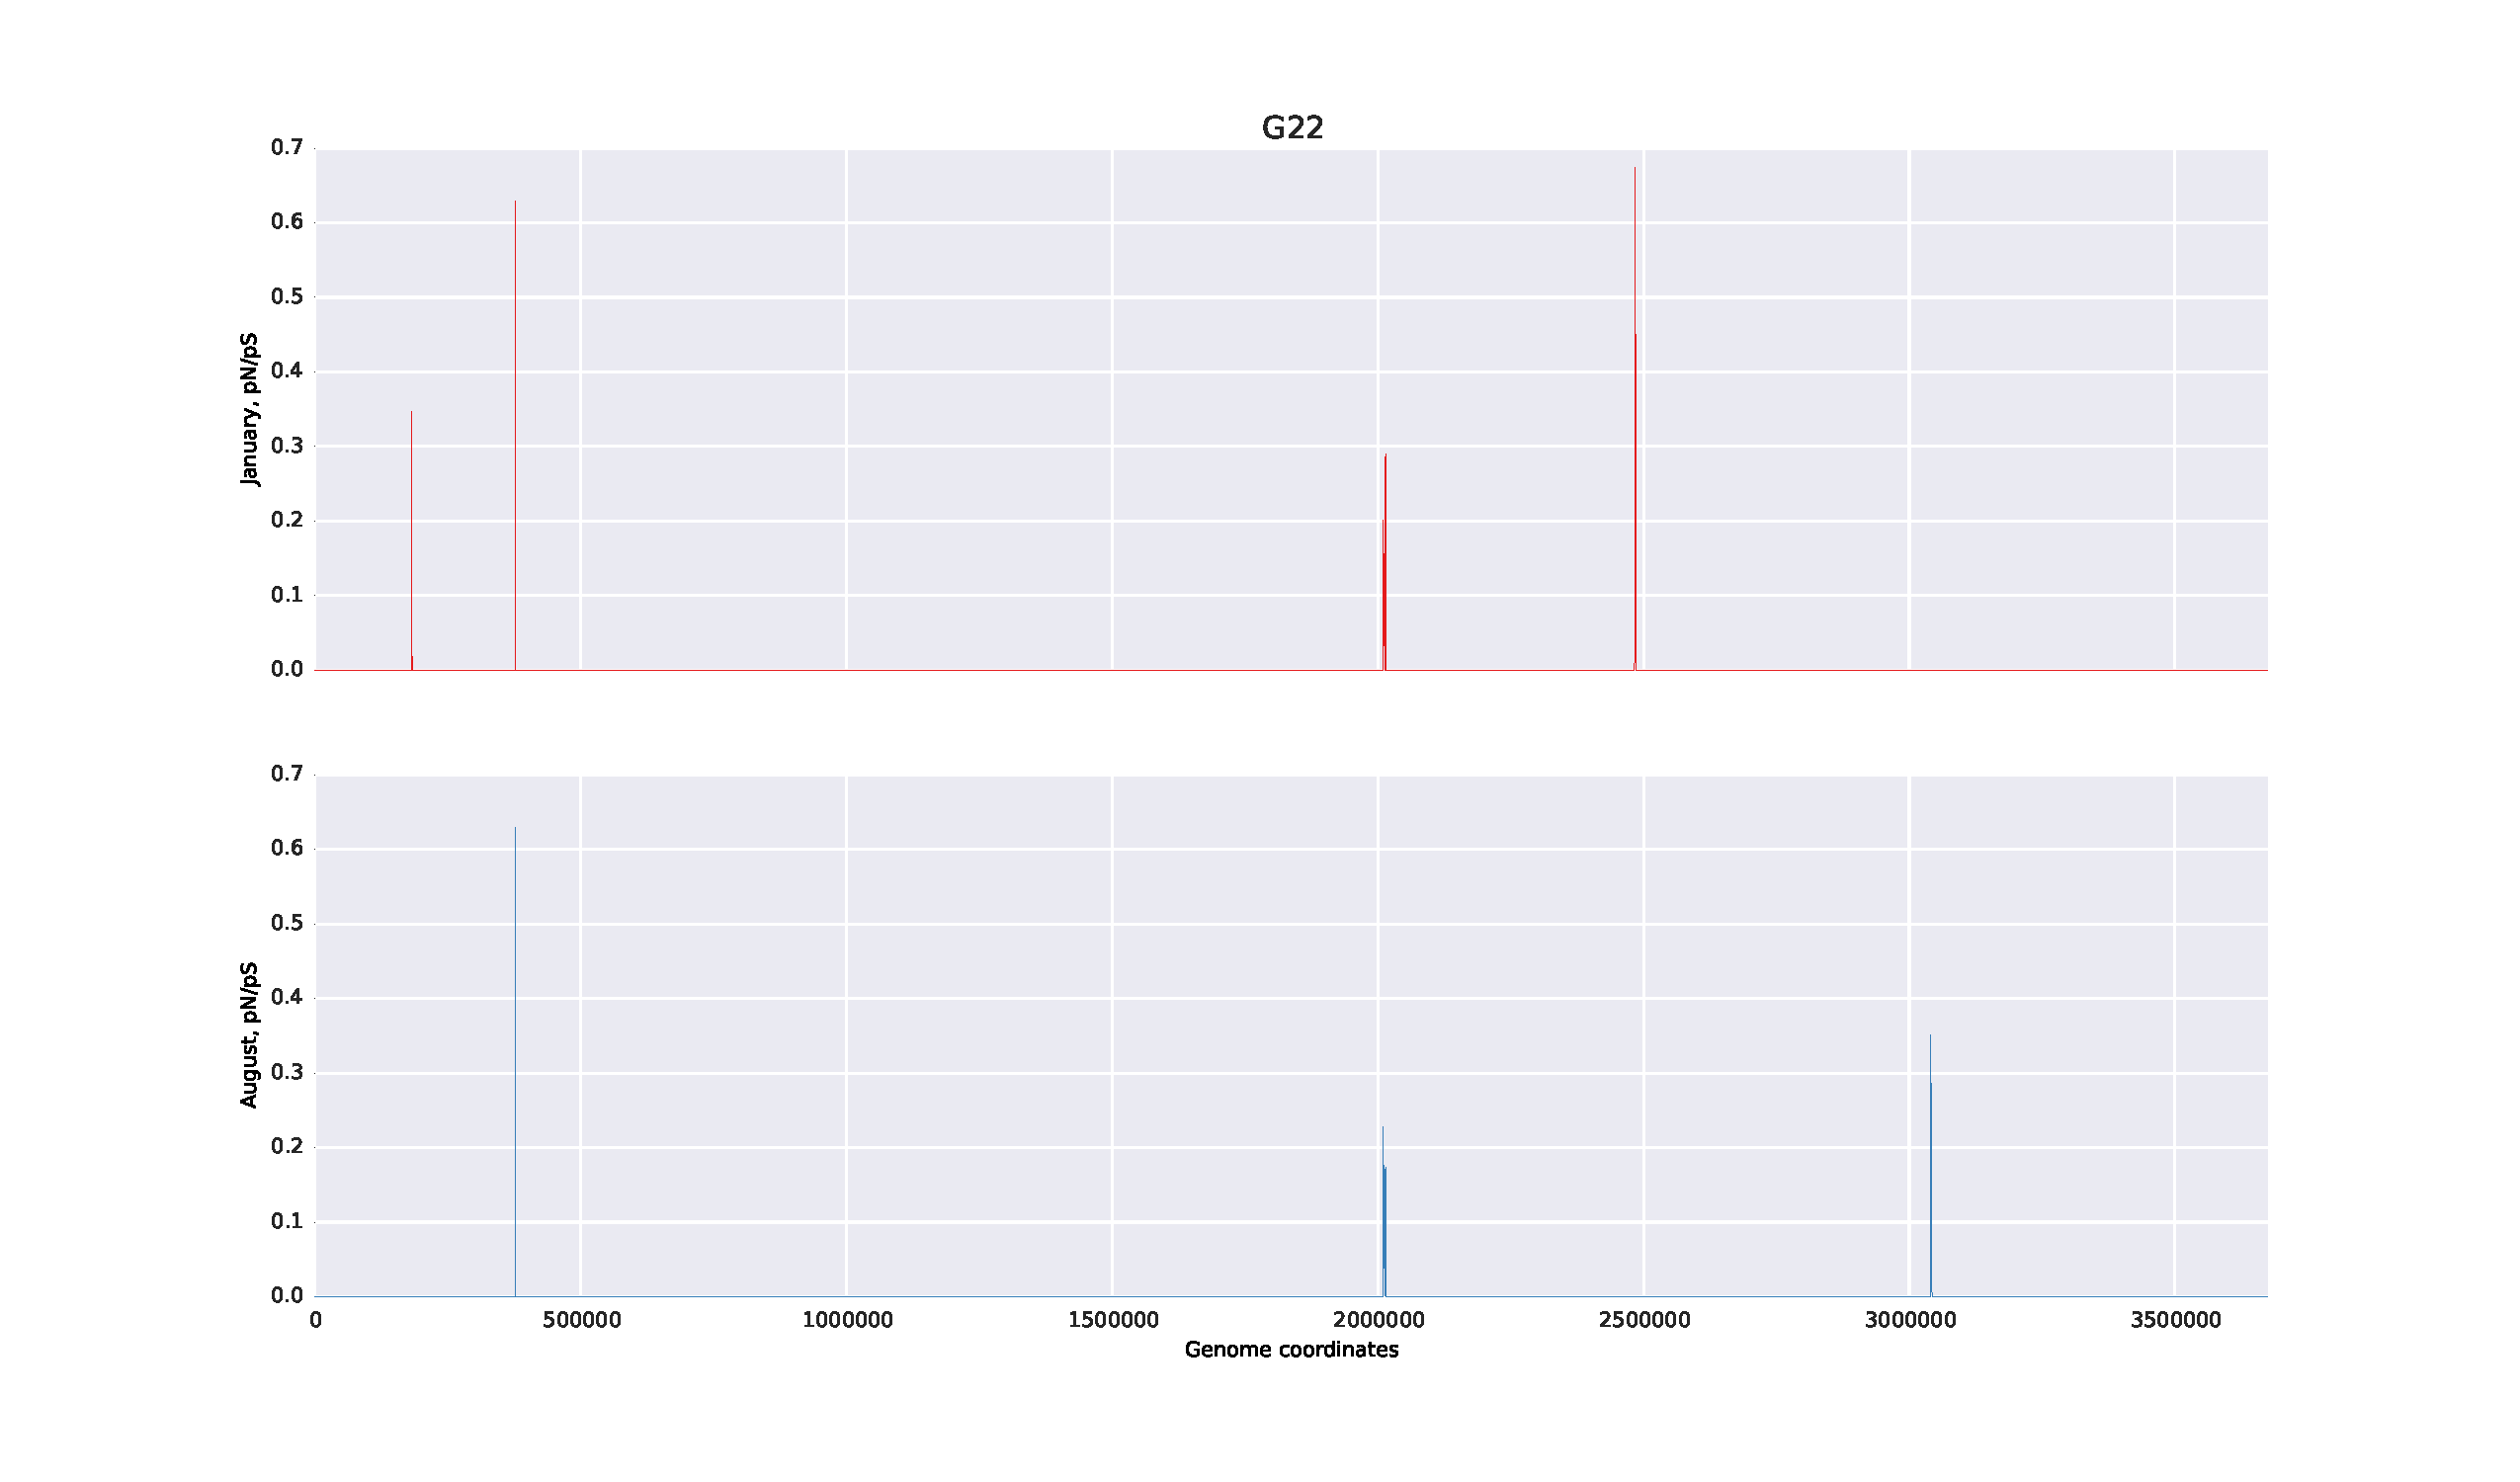
\includegraphics[width=\textwidth,height=\textheight,keepaspectratio]{Chapter5/Figures/pn_ps_plots/G22_pNpS_density.pdf}
  \caption{pN/pS values for each gene in the G22 genome. Top panel shows the values using the reads from the January samples. Bottom panel shows the values using the reads from the August sample}
  \label{G22_pNpS}
\end{figure}
